\documentclass[final,12pt]{colt2018} 

% The following packages will be automatically loaded:
% amsmath, amssymb, natbib, graphicx, url, algorithm2e

%%%
% Packages
\usepackage{amssymb,amsmath,sectsty,url}
%\usepackage[letterpaper,hmargin=1.0in,vmargin=1.0in]{geometry}
%\usepackage[dvips,colorlinks,linkcolor=blue,citecolor=blue,filecolor=blue,urlcolor=blue]{hyperref}
%\usepackage[pdftex,colorlinks,linkcolor=blue,citecolor=blue,filecolor=blue,urlcolor=blue]{hyperref}
%\usepackage[dvips,colorlinks,linkcolor=black,citecolor=black,filecolor=black,urlcolor=black]{hyperref}
%\usepackage[colorlinks,linkcolor=black,citecolor=black,filecolor=black,urlcolor=black]{hyperref}
\usepackage{cleveref}
\usepackage{color}
\usepackage[boxed]{algorithm}
%\usepackage[margin=20pt,font=small,labelfont=bf]{caption}
\pagestyle{plain}

\usepackage{tikz}
\usepackage{graphicx}
\usepackage{nicefrac}
\usepackage{aliascnt}

\newcommand{\aref}[1]{\autoref{#1}}

\numberwithin{theorem}{section}

%General
\newcommand{\abs}[1]{\left|#1\right|} 
\newcommand{\norm}[1]{\lVert#1\rVert}

%Probability
\def\E{\mathbb E}
\newcommand{\Exp}{\mathop{\mathrm E}\displaylimits} % expectation
\newcommand{\Var}{{\bf Var}}
\newcommand{\Cov}{{\bf Cov}}
\newcommand{\1}{{\rm 1\hspace*{-0.4ex}%

\rule{0.1ex}{1.52ex}\hspace*{0.2ex}}}

%Algebraic Structures
\newcommand{\U}{\mathbf U}
\newcommand{\N}{\mathbb N}
\newcommand{\R}{\mathbb R}
\newcommand{\Z}{\mathbb Z}
\newcommand{\C}{\mathbb C}
\newcommand{\F}{\mathbb F}
\newcommand{\GF}{\mathbb{GF}}
\newcommand{\B}{\{ 0,1 \}}
\newcommand{\BM}{\{ -1,1 \}}

% Misc
\newcommand\polylog[1]{\ensuremath{\mathrm{polylog}\left(#1\right)}}
\newcommand\argmin{\ensuremath{\mathrm{argmin}}}
\newcommand\qed{\hfill$\blacksquare$}

%%%

\newaliascnt{claim}{theorem}
\newtheorem{claim}[claim]{Claim}
\aliascntresetthe{claim}
\crefname{claim}{Claim}{Claims}

%\newaliascnt{lemma}{theorem}
%\newtheorem{lemma}[lemma]{Lemma}
%\aliascntresetthe{lemma}
%\crefname{lemma}{Lemma}{Lemmas}

\title[Approximate Nearest Neighbors in Limited  Space]{Approximate Nearest Neighbors in Limited  Space}
\usepackage{times}
 % Use \Name{Author Name} to specify the name.
 % If the surname contains spaces, enclose the surname
 % in braces, e.g. \Name{John {Smith Jones}} similarly
 % if the name has a "von" part, e.g \Name{Jane {de Winter}}.
 % If the first letter in the forenames is a diacritic
 % enclose the diacritic in braces, e.g. \Name{{\'E}louise Smith}

 % Two authors with the same address
  % \coltauthor{\Name{Author Name1} \Email{abc@sample.com}\and
  %  \Name{Author Name2} \Email{xyz@sample.com}\\
  %  \addr Address}

 % Three or more authors with the same address:
 % \coltauthor{\Name{Author Name1} \Email{an1@sample.com}\\
 %  \Name{Author Name2} \Email{an2@sample.com}\\
 %  \Name{Author Name3} \Email{an3@sample.com}\\
 %  \addr Address}


 % Authors with different addresses:
 \coltauthor{\Name{Piotr Indyk} \Email{indyk@mit.edu}\\
 \addr CSAIL, MIT
 \AND
 \Name{Tal Wagner} \Email{talw@mit.edu}\\
 \addr CSAIL, MIT
 }

\begin{document}

\maketitle

\begin{abstract}
We consider the $(1+\epsilon)$-approximate nearest neighbor search problem: given a set $X$ of $n$ points in a $d$-dimensional space, build a data structure that, given any query point  $y$,  finds a point $x \in X$ whose distance to $y$ is at most $(1+\epsilon) \min_{x \in X} \|x-y\|$ for an accuracy parameter $\epsilon \in (0,1)$.  Our main result is a data structure that occupies only $O(\epsilon^{-2} n \log(n) \log(1/\epsilon))$
bits of space, assuming all point coordinates are integers in the range  $\{-n^{O(1)} \ldots n^{O(1)}\}$, i.e., the coordinates have $O(\log n)$ bits of precision. This improves over the best previously known space bound of         $O(\epsilon^{-2} n \log(n)^2)$, obtained via the randomized dimensionality reduction method of \cite{johnson1984extensions}.  We also consider the more general problem of estimating all distances from a collection of query points to all data points $X$, and provide almost tight upper and lower bounds for the space complexity of this problem. 
\end{abstract}

\begin{keywords}
nearest neighbor, quantization, distance estimation, metric compression, distance sketches, dimension reduction
\end{keywords}

% !TeX root = main.tex
\section{Introduction}
\label{sec:intro}
Generative models are often trained in an unsupervised fashion, fitting a model $q$ to a set of observed data $x_P \subseteq X$ drawn iid from some true distribution $p$ on $x\in X$. Now, of course $p$ may not exactly belong to family $Q$ of probability distributions being fit, whether $Q$ consists of Gaussians mixture models, Markov models, or even neural networks of bounded size. We first discuss the limitations of generative modeling without feedback, and then discuss our model and results.

%\subsection{Limitations of Generative Modeling from Positive Examples Alone}
Consider fitting a generative model on a text corpus consisting partly of poetry written by four-year-olds and partly of mathematical publications from the {\em Annals of Mathematics}. Suppose that learning to generate a poem that looks like it was written by a child was easier than learning to generate a novel mathematical article with a correct, nontrivial statement. If the generative model pays a high price for generating unrealistic examples, then it may be better off learning to generate children's poetry than mathematical publications. However, without negative feedback, it may be difficult for a neural network or any other model to know that the mathematical articles it is generating are stylistically similar to the mathematical publications but do not contain valid proofs.\footnote{This is excluding clearly fake articles published without proper review in lower-tier venues \citep{LabbeL13}.} 

As a simpler example, the classic Markovian ``trigram model'' of natural language assigns each word a fixed probability conditioned only on the previous two words. Prior to recent advances in deep learning, for decades the trigram model and its variant were the workhorses of language modeling, assigning much greater likelihood to natural language corpora than numerous linguistically motivated grammars and other attempts \citep{Rosenfeld00}. However, text sampled from a trigram is typically nonsensical, e.g., the following text was randomly generated from a trigram model fit on a corpus of text from the Wall Street Journal \citep{JurafskyM09}:
\begin{quote}
They also point to ninety nine point six billion dollars from two hundred
four oh six three percent of the rates of interest stores as Mexico and
gram Brazil on market conditions. 
\end{quote}

In some applications, like text compression using a language model \citep{WittenNC87}, maximizing likelihood is equivalent to optimizing compression. However, in many  applications involving generation, such nonsense is costly and unacceptable. Now, of course it is possible to always generate valid data by returning random training examples, but this is simply overfitting and not learning. Alternatively, one could incorporate human-in-the-loop feedback such as through crowdsourcing, into the generative model to determine what is a valid, plausible sentence.

In some domains, validity could be determined automatically. Consider a Markovian model of a well-defined concept such as mathematical formulas that compile in \LaTeX{}. Now, consider a $n$-gram Markovian character model which the probability of each subsequent character is determined by the previous $n$ characters. For instance, the expression \$\{2+\{x-y\}\$ is invalid in \LaTeX{} due to mismatched braces. For this problem, a \LaTeX{} compiler may serve as a validity oracle. Various $n$-gram models can be fit which only generate valid formulas. To address mismatched braces, for example, one such model would ensure that it always closed braces within $n$ characters of opening, and had no nested braces. While an $n$-gram model will not perfectly model the true distribution over valid \LaTeX{} formulas, for certain generative purposes one may prefer an $n$-gram model that generates valid formulas over one that assigns greater likelihood to the training data but generates invalid formulas. 

Figure \ref{fig:rectangle} illustrates a simple case of learning a rectangle model for data which is not uniform over a rectangle. A maximum likelihood model would necessarily be the smallest rectangle containing all the data, but most examples generated from this distribution may be invalid. Instead a smaller rectangle, as illustrated in the figure, may be desired.

\begin{figure}[h]\label{fig:rectangle}
\centering
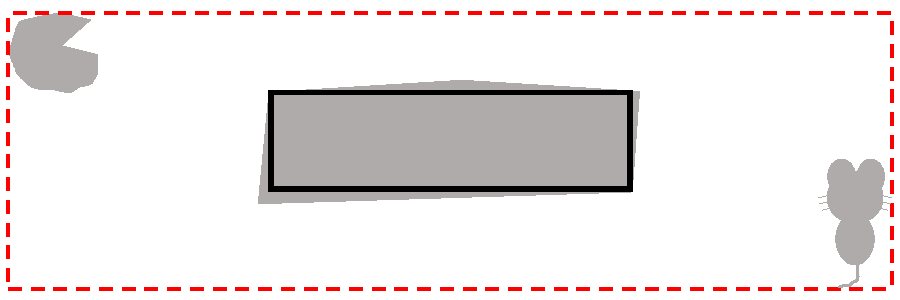
\includegraphics[width=3in]{fig.pdf}
\caption{Example where the underlying distribution $p$ is uniform over the (gray) valid regions. The solid rectangle maximizes our objective since it does not output nonsense (is supported only within the grey matter) and is closest to the $p$ (covers the maximum amount of grey matter). In contrast, the standard maximum likelihood (dashed red) rectangle must fully contain the observed samples, thus generating invalid points most of the time.  }
\end{figure}

Motivated by these observations, we evaluate a generative model $q$ on two axes. First is {\em coverage}, which is related to the probability assigned to future examples drawn from the true distribution $p$. Second is {\em validity}, defined as the probability that random examples generated from $q$ meet some validity requirement. Formally, we measure coverage in terms of a bounded {\em loss}:
$$\Loss(p,q)=\E_{x \sim p}[L(q_x)],$$
where $L:[0,1]\rightarrow [0,M]$ is a bounded decreasing function such as the capped log-loss $L(q_x)=\min(M, \log 1/q_x)$. % or $L(q_x)=\log 1/(q_x+\exp(-M))$. 
A bounded loss has the advantages of being efficiently estimable, and also it enables a model to assign 0 probability to one example (e.g., an outlier or error) if it greatly increases the likelihood of all other data. Validity is defined with respect to a set $V \subseteq X$, and $q(V)$ is the probability that a random example generated from $q$ lies within $V$. 

Clearly, there is a tradeoff between coverage and validity. We first focus on the case of (near) perfect validity. A Valid Generative Modeling (VGM) algorithm if it outputs, for a family of distributions $Q$ over $X$, if it outputs $\hat{q}$ with (nearly) perfect validity and whose loss is nearly as good as the loss of the best valid $q\in Q$. More precisely, $A$ is a VGM learner of $Q$ if for any nonempty valid subset $V \subseteq X$, any probability distribution $p$ over $V$, and any $\eps>0$, $A$ uses $n$ random samples from $p$ and makes $m$ membership oracle calls to $V$ and outputs a distribution $\hat{q}$ such that, $$\Loss(p, \hat{q}) \leq \min_{q \in Q: q(V)=1}\Loss(p,q) + \eps ~\text{ and }~\hat{q}(V)\geq 1-\eps.$$ 
We aim for our learner to be sample and query efficient, requiring that $n$ and $m$ are polynomial in $M, 1/\eps$ and a measure of complexity of our distribution class $Q$.
Furthermore, we would like our algorithms to be computationally efficient, with a runtime polynomial in the size of the data, namely the $n + m$ training examples. 
A more formal description of the problem is available in Section~\ref{sec:problem}.

$A$ is said to be {\em proper} if it always outputs $\hat{q}\in Q$ and {\em improper} otherwise.
In Section~\ref{sec:impossibility}, we first show that efficient proper learning for VGM is impossible. This is an information-theoretic result, meaning that even given infinite runtime and positive samples, one still cannot solve the VGM problem. Interestingly, this is different from binary classification, where it is possible to statistically learn from iid examples without a membership oracle.

Our first main positive result is an efficient (improper) learner for VGM. The algorithm relies on a subroutine that solves the following {\em Generative Modeling with Negatives} (GMN) problem: given sets $X_P, X_N \subset X$ of positive and negative examples, find the probability distribution $q \in Q$ which minimizes $\sum_{x \in X_P} L(q(x))$ subject to the constraint that $q(X_N)=0$. For simplicity, we present our algorithm for the case that the distribution family $Q$ is finite, giving sample and query complexity bounds that are logarithmic in terms of $|Q|$. However, as we show in Section~\ref{sec:infinite-families}, all of our results extend to infinite families $Q$. It follows that if one has a computationally efficient algorithm for the GMN problem for a distribution family $Q$, then our reduction gives a computationally efficient VGM learning algorithm for $Q$.

Our second positive result is an algorithm that minimizes $\Loss(p,q)$ subject to a relaxed validity constraint comparing against the optimal distribution that has validity $q(V)$ at least $1-\alpha$ for some $\alpha>0$. We show in Section~\ref{sec:partial-validity} that even in this more general setting, it is possible to obtain an algorithm that is statistically efficient but may not be computationally efficient. An important open question is whether there exists a computationally efficient algorithm for this problem when given access to an optimization oracle, as was the case for our algorithm for VGM.

\subsection{Related Work}
\cite{KearnsMRRSS94} showed how to learn distributions from positive examples in the realizable setting, i.e., where the true distribution is assumed to belong to the class being learned. In the same sense as their work is similar to PAC learning \citet{Valiant84} of distributions, our work is like agnostic learning \citet{KearnsSS94} in which no assumption on the true distribution is made. 

Generative Adversarial Networks (GANs)~\cite{GoodfellowPMXWOCB14} are an approach for generative modeling from positive examples alone, in which a generative model is trained against a discriminator that aims to distinguish real data from generated data. In some domains, GANs have been shown to outperform other methods at generating realistic-looking examples. Several shortcomings of GANs have been observed \citet{AroraRZ18}, and GANs are still subject to the theoretical limitations we argue are inherent to any model trained without a validity oracle. 

In supervised learning, there is a rich history of learning theory with various types of queries, including membership which are not unlike our (in)validity oracle. Under various assumptions, queries have been shown to facilitate the learning of complex classes such as finite automata \citet{Angluin88} and DNFs \citet{Jackson97}. See the survey of \cite{Angluin92} for further details.  Interestingly, \cite{Feldman09} has shown that for agnostic learning, i.e., without making assumptions on the generating distribution, the addition of membership queries does not enhance what is learnable beyond random examples alone. 
Supervised learning also has a large literature around active learning, showing how the ability to query examples reduces the sample complexity of many algorithms. See the survey of \cite{Hanneke14}. Note that the aim here is typically to save examples and not to expand what is learnable.
 
More sophisticated models, e.g., involving neural networks, can mitigate the invalidity problem as they often generate more realistic natural language and have even been demonstrated to generate \LaTeX{} that nearly compiles \citep{Karpathy15} or nearly valid Wikipedia markdown. However, longer strings generated are unlikely to be valid. For example, \cite{Karpathy15} shows generated markdown which includes:
\begin{quote}
==Access to ''rap===
The current history of the BGA has been [[Vatican Oriolean Diet]], British Armenian, published in 1893.  While actualistic such conditions such as the [[Style Mark Romanians]] are still nearly not the loss.
\end{quote}

Even ignoring the mismatched quotes and equal signs, note that this example has two so-called ``red links'' to two pages that do not exist. Without checking, it was not obvious to us whether or not Wikipedia had pages titled {\em Vatican Oriolean Diet} or {\em Style Mark Romanians}. In some applications, one may or may not want to disallow red links. In the case that they are considered valid, one may seek a full generative model of what might plausibly occur inside of brackets, as the neural network has learned in this case. If they are disallowed, a model might memorize links it has seen but not generate new ones. A validity oracle can help the learner identify what it should avoid generating.

 In practice, \cite{KusnerPH17} discuss how generative models from neural networks (in particular autoencoders) often generate invalid sequences. 
\cite{JanzWPKH18} learn the validity of examples output by a generative model using oracle feedback. 

\usepackage[papersize={17cm,24cm},margin=22mm,top=17mm,headsep=5mm]{geometry} 
%\usepackage[papersize={17cm,24cm},margin=13mm,top=17mm,headsep=5mm]{geometry} 
%\usepackage[utf8]{inputenc}
\usepackage{xltxtra} % extras for XeLaTeX
\usepackage{unicode-math}
\usepackage{amsmath}
\usepackage{amsthm}
\usepackage{enumerate}
\usepackage{verbatim} % verbatim input
\usepackage{titling} % customize title
\usepackage{csquotes} % context sensitive quotes
\usepackage{upquote} % allow correct quotes in verbatim
\usepackage[bottom]{footmisc} % put footnotes down at the bottom margin
\usepackage[svgnames]{xcolor} % color pictures with SVG names
\usepackage{graphicx} % \includegraphics
\usepackage[noend]{algpseudocode}
\usepackage[linesnumbered,ruled]{algorithm2e}
\usepackage{thmtools}
\usepackage{thm-restate}
\usepackage{authblk}
%\usepackage{hyperref}
%\usepackage{optidef}
%\usepackage{enumitem} % customize lists
%\setitemize{noitemsep,topsep=0pt,parsep=0pt,partopsep=0pt}
%\setitemize{itemsep=2pt,topsep=4pt,parsep=0pt,partopsep=0pt}
%\usepackage{covington}  % for numbered linguistic examples


%\usepackage[english]{babel} % multilinguality
\usepackage{polyglossia} % newer alternative to babel
\setdefaultlanguage{english} % see http://ctan.uib.no/macros/xetex/latex/polyglossia/polyglossia.pdf
\setmainfont[Mapping=tex-text,Ligatures=TeX,Scale=1.0]{Linux Libertine O} 
\setmonofont[Mapping=tex-text,Scale=MatchLowercase,LetterSpace=-2.0]{DejaVu Sans Mono}
%\setmathfont{Cambria Math}
%\setmathfont[math-style=upright,vargreek-shape=unicode]{Neo Euler}
%\setmathfont{Linux Libertine O}
\renewcommand{\baselinestretch}{1.04} % stretch distance between baselines
\frenchspacing % reduce space after sentence-final punctuation
\date{}
\setlength{\parindent}{1em}
\clubpenalty = 10000
\widowpenalty = 10000
\hfuzz = 2pt  % No warnings about margin overhangs less than this amount.
%\setlength{\belowcaptionskip}{-1.2em}
%Theorem Repeat solutions

%\usepackage[backend=biber, style=authoryear, citestyle=authoryear-comp, maxcitenames=2, maxbibnames=50, language=auto, isbn=false, url=false]{biblatex} % new alternative to bibtex
%\setlength{\bibhang}{\parindent}
%\usepackage[breaklinks,colorlinks,urlcolor=black,citecolor=black,linkcolor=black]{hyperref} % pagebackref incompatible with biblatex

%\usepackage[compact,noindentafter]{titlesec} % customize section headings
%\titlespacing{\section}{0pt}{2.7mm}{1.5mm} % left indent, space before, space after
%\titlespacing{\subsection}{0pt}{2mm}{1pt}
%\titlespacing{\subsubsection}{0pt}{1.2mm}{0.5pt}

%\newcommand\Volume{N} % BeLLS Volume number
%\newcommand\Voleditors{Jan Editor and Ed Janitor}
%\newcommand\Voltitle{The book title}
%\newcommand\VolISBN{N}
%\newcommand\VolDOI{N}

\usepackage{natbib}
%\usepackage{fullname}
%\bibliographystyle{chicago} % chicago or spbasic or spmpsci or spphys
\bibliographystyle{unsrt}
%\setlength{\bibhang}{-0.5em}
%\setlength{\bibsep}{0mm}
%\let\bibfont=\small

% footnote without number
\newcommand\blfootnote[1]{
  \begingroup
  \renewcommand\thefootnote{}\footnote{\hspace{-2.4em} #1}%
  \addtocounter{footnote}{-1}
  \endgroup
}

% customize title
%\renewcommand{\maketitle}
%  {\bgroup\setlength{\parindent}{0pt}
%   \begin{flushleft}
%    \textbf{\LARGE{\ \\ \vspace{20mm}\strut\thetitle\strut}\vspace{2mm}}
%    
%    {\Large\theauthor}
%  \end{flushleft}\egroup\vspace{18mm}
%}

% customize abstract
\renewenvironment{abstract}
  {\noindent\small %\quotation
  {\noindent{\large\textbf\abstractname. }%\par\nobreak\smallskip
  \thispagestyle{plain}
  %\blfootnote{In: \emph{Volume title,} edited by Jan Editor and Ed Janitor. BeLLS Vol. N (2017), DOI N. Open Access under the terms of CC-BY-NC-4.0.}
  }}
  {}
    
% command in which to embed tabular material in numbered example
% use: \begin{example}\extab\begin{tabular ...
\newcommand{\extab}[2][-0.69\baselineskip]{ 
   \parbox[t]{.9\textwidth}{
     \setlength{\tabcolsep}{1.3pt} % use small space between columns
     \vspace{#1}
     #2
    }
}

% command to put ref in parentheses
\newcommand{\refp}[1]{(\ref{#1})}

% customize page headers
\usepackage{fancyhdr}
\pagestyle{fancy}
\renewcommand{\headrulewidth}{0.4pt}
\fancyhead{}  \cfoot{\thepage}%\fancyfoot{\thepage} %clear
\makeatletter % necessary for commands with @
  \fancyhead[RO]{\small\textit{\@title}}
  %\fancyhead[LE]{\small\textit{Peter L. Bartlett \& Niladri S. Chatterji}}
  \fancyhead[LE]{\small\textit{X. Cheng, N.S. Chatterji, P.L. Bartlett \& M.I. Jordan}}
\makeatother
%\fancyhead[RE]{\small BeLLS Vol. \Volume}
 % no footer
\setlength{\headheight}{20.68pt} % room for two lines
\fancypagestyle{plain}{% first page of chapter
 %\fancyhead[L]{}
 %\fancyhead[L]{\footnotesize In: \emph{Volume title,} edited by Jan Editor and Ed Janitor. BeLLS Vol. N (2017), DOI N. Open Access under the terms of CC-BY-NC-4.0.} % comment to keep the normal header
  \fancyhead[C,R]{}
  \renewcommand{\headrulewidth}{0pt} % comment to keep rule
  \fancyfoot{} % comment to put page number at bottom
  }
  
  %user defined commands
  \newcommand*\Mirr[1]{\textsc{Mirr} (#1)}
\newcommand*\Wd[0]{\textit{W}_2}
\newcommand*\dd[2]{\frac{\partial #1}{\partial #2}}
\newcommand*\x[0]{\textbf{x}}
\newcommand*\stein[1]{\mathcal{A}_{#1}}
\newcommand*\w[0]{\textbf{w}}
\newcommand*\at[2]{\left.#1\right|_{#2}}
\newcommand*\ps[0]{p^*}
\newcommand*\del[0]{\partial}
\newcommand*\R[0]{\mathbb{R}}
\newcommand*\Z[0]{\mathbb{Z}}
\renewcommand*\div[0]{\nabla \cdot}
\newcommand*\ddt[0]{\frac{d}{d t}}
\newcommand*\dds[0]{\frac{d}{d s}}
\newcommand*\ddp[1]{\frac{\delta #1}{\delta p}}
\newcommand*\tr[0]{\text{tr}}
\newcommand*\KL[2]{\mathcal{KL}\left(#1\|#2\right)}
\newcommand*\lin[1]{\langle #1\rangle}
\newcommand*\E[1]{\mathbb{E}\left[#1\right]}
\newcommand*\Ep[2]{\mathbb{E}_{#1}\left[#2\right]}
\newcommand*\grad[3]{\mathcal{D}_{#1}(#2,#3)}
\newcommand*\slope[1]{\|\mathcal{D}_{#1}\|}
\newcommand*\md[1]{\|\frac{d}{dt}#1\|}
\newcommand*\ap[2]{\tilde{#1}_{#2}}
\newcommand*\F[0]{\mathcal{F}}
\newcommand*\D[0]{\mathcal{D}}
\renewcommand*\H[0]{\mathcal{H}}
\newcommand*\Pspace[0]{\mathscr{P}}
\newcommand*\Uspace[0]{\mathbb{U}}
\renewcommand*\t[1]{\tilde{#1}}
\renewcommand*\d[0]{\text{d}}
\newcommand*\ot[1]{#1^{\perp}}
\newcommand*\proj[0]{\text{Proj}}
\newcommand\numberthis{\addtocounter{equation}{1}\tag{\theequation}}
\newcommand*\lrb[1]{\left[#1\right]}
\newcommand*\lrp[1]{\left(#1\right)}
\newcommand*\eu[1]{\left\| #1\right\|}
\renewcommand*\div[0]{\nabla \cdot}
\renewcommand*\H[0]{\mathcal{H}}
\renewcommand*\t[1]{\tilde{#1}}
\renewcommand*\d[0]{\delta}
\newcommand*\xt[0]{\tilde{x}}
\newcommand*\vt[0]{\tilde{v}}
\newcommand*\pt[0]{\tilde{p}}
\newcommand*\qt[0]{\tilde{q}}
\newcommand*\Phit[0]{\tilde{\Phi}}
%NewSymbols
\def\ci{\perp\!\!\!\perp}
\def\half{\frac{1}{2}}
\def\lv{\lVert}
\def\rv{\rVert}
\def\ke{\mathcal{E}_K}

\section{Basic Sketch}\label{sec:sketch}

In this section we describe the basic data structure (generated by Alice) used for all of our results.
% Below we describe Alice's sketching algorithm. Assume w.l.o.g.~that the minimum distance within $X\cup Y$ is $1$ and the diameter is $\Phi$. 
The data structure augments the representation from~\cite{indyk2017near}, which we will now reproduce.
For the sake of readability, the notions from the latter paper (tree construction via hierarchical clustering, centers, ingresses and surrogates) are interleaved with the new ideas introduced in this paper (top-out compression, grid quantization and surrogate hashing).
Proofs in this section are deferred to Appendix~\ref{sec:sketch_proofs}.

%\textcolor{blue}{Changes from the SODA construction are colored in blue.}

\subsection{Hierarchical Clustering Tree}
The sketch consists of an annotated hierarchical clustering tree, which we now describe with our modified ``top-out compression'' step.

\paragraph{Tree construction}
We construct the inter-link hierarchical clustering tree of $X$: In the bottom level (numbered $0$) every point is a singleton cluster, and level $\ell>0$ is formed from level $\ell-1$ by recursively merging any two clusters whose distance is at most $2^\ell$, until no two such clusters are present.
We repeat this until level $\lceil\log(2\sqrt d\Phi)\rceil$, even if all points in $X$ are already joined in one cluster at a lower level.
%Note that every level in the tree induces a partition of $X$ into the clusters associated with the nodes at that level.
The following observation is immediate.
\begin{lemma}\label{lmm:separation}
If $x,x'\in X$ are in different clusters at level $\ell$, then $\norm{x-x'}\geq2^\ell$.
\end{lemma}

\paragraph{Notation}
Let $T^*$ denote the tree.
For every tree node $v$, we denote its level by $\ell(v)$, its associated cluster by $C(v)\subset X$, and its cluster diameter by $\Delta(v)$. For a point $x_i\in X$, let $\mathrm{leaf}(x_i)$ denote the tree leaf whose associated cluster is $\{x_i\}$.


\paragraph{Top-out compression}
The~\emph{degree} of a node in $T^*$ is its number of children.
A~\emph{$1$-path with $k$ edges} in  $T^*$ is a downward path $u_0,u_1,\ldots,u_k$, such that (i) each of the nodes $u_0,\ldots,u_{k-1}$ has degree $1$, (ii) $u_k$ has degree either $0$ or more than $1$, (iii) if $u_0$ is not the root of $T^*$, then its ancestor has degree more than $1$.

For every node $v$ denote $\Lambda(v) := \log(\Delta(v)/(2^{\ell(v)}\epsilon))$. 
If $v$ is the bottom of a $1$-path with more than $\Lambda(v)$ edges, we replace all but the bottom $\Lambda(v)$ edges with a~\emph{long edge}, and annotate it by the length of the path it represents.
More precisely, if the downward $1$-path is $u_0,\ldots,u_k=v$ and $k>\Lambda(v)$, then we connect $u_0$ directly to $u_{k-\Lambda(v)}$ by the long edge, and the nodes $u_1,\ldots,u_{k-\Lambda(v)-1}$ are removed from the tree, and the long edge is annotated with length $k-\Lambda(v)$.

\begin{lemma}\label{lmm:tree_size}
The compressed tree has $O(n\log(1/\epsilon))$ nodes.
\end{lemma}


We henceforth refer only to the compressed tree, and denote it by $T$.
However, for every node $v$ in $T$, $\ell(v)$ continues to denote its level before compression (i.e., the level where the long edges are counted according to their lengths).
We partition $T$ into~\emph{subtrees} by removing the long edges.
Let $\mathcal F(T)$ denote the set of subtrees.

\begin{lemma}\label{lmm:subtree_root}
Let $v$ be the bottom node of a long edge, and $x,x'\in C(v)$. Then $\norm{x-x'}\leq2^{\ell(v)}\epsilon$.
\end{lemma}

\begin{lemma}\label{lmm:subtree_leaf}
Let $u$ be a leaf of a subtree in $\mathcal F(T)$, and $x,x'\in C(u)$. Then $\norm{x-x'}\leq2^{\ell(u)}\epsilon$.
\end{lemma}


\subsection{Surrogates}
The purpose of annotating the tree is to be able to recover a list of~\emph{surrogates} for every point in $X$.
A surrogate is a point whose location approximates $x$.
Since we will need to compare $x$ to a new query point, which is unknown during sketching, we define the surrogates to encompass a certain amount information about the absolute point location, by hashing a coarsened grid quantization of a representative point in each subtree.

\paragraph{Centers}
With every tree node $v$ we associate an index $c(v)\in[n]$ such that $x_{c(v)}\in C(v)$, and we call $x_{c(v)}$ the~\emph{center} of $C(v)$.
The centers are chosen bottom-up in $T$ as follows.
For a leaf $v$, $C(v)$ contains a single point $x_i\in X$, and we set $c(v)=i$. 
For a non-leaf $v$ with children $u_1,\ldots,u_k$, we set $c(v)=\min\{c(u_i):i\in[k]\}$.

\paragraph{Ingresses}
Fix a subtree $T'\in\mathcal F(T)$.
To every node $u$ in $T'$, except the root, we will now assign an~\emph{ingress} node, denoted $\mathrm{in(u)}$.
Intuitively this is a node in the same subtree whose center is close to $u$, and the purpose is to store the location of $u$ by its quantized displacement from that center (whose location will have been already stored, by induction).

We will now assign ingresses to all children of a given node $v$. (Doing this for every $v$ in $T'$ defines ingresses for all nodes in $T'$ except its root.) Let $u_1,\ldots,u_k$ be the children of $v$, and w.l.o.g.~$c(v)=c(u_1)$. Consider the graph $H_v$ whose nodes are $u_1,\ldots,u_k$, and $u_i,u_j$ are neighbors if there are points $x\in C(u_i)$ and $x'\in C(u_j)$ such that $\norm{x-x'}\leq2^{\ell(v)}$. By the tree construction, $H_v$ is connected. We fix an arbitrary spanning tree $\tau(v)$ of $H_v$ which is rooted at $u_1$.

For $u_1$ we set $\mathrm{in}(u_1):=v$. For $u_i$ with $i>1$, let $u_j$ be its (unique) direct ancestor in the tree $\tau(v)$. Let $x\in C(u_j)$ be the closest point to $C(u_i)$ in $C(u_j)$. Note that in $T$ there is a downward path from $u_j$ to $\mathrm{leaf}(x)$. Let $u_x$ be the bottom node in that path that belongs to $T'$. (Equivalently, $u_x$ is the bottom node on that downward path that is reachable from $u$ without traversing a long edge.) We set $\mathrm{in}(u_i):=u_x$.

\paragraph{Grid net quantization}
Assume w.l.o.g.~that $\Phi$ is a power of $2$.
We define a hierarchy of grids aligned with $\{-\Phi \ldots \Phi\}^d$ as follows.
We begin with the single hypercube whose corners are $(\pm\Phi, \ldots, \pm\Phi)^d$.
We generate the next grid by halving along each dimension, and so on.
For every $\gamma>0$, let $\mathcal{N}_\gamma$ be the coarsest grid generated, whose cell side is at most $\gamma/\sqrt{d}$. Note that every cell in $\mathcal{N}_\gamma$ has diameter at most $\gamma$.
For a point $x\in\R^d$, we denote by $\mathcal{N}_\gamma[x]$ the closest corner of the grid cell containing it.

We will rely on the following fact about the intersection size of a grid and a ball; see, for example, \cite{har2012approximate}.

\begin{claim}\label{clm:gridball}
For every $\gamma>0$, the number of points  in $\mathcal N_\gamma$ at distance at most $2\gamma$ from any given point, is at most $O(1)^d$.
\end{claim}


\paragraph{Surrogates}
Fix a subtree $T'\in\mathcal F(T)$. With every node $v$ in $T'$ we will now associate a~\emph{surrogate} $s^*(v)\in\R^d$.
Define the following for every node $v$ in $T'$:
\[
  \gamma(v) = 
  \begin{cases}
  \left(5 + \lceil\frac{\Delta(v)}{2^{\ell(v)}}\rceil\right)^{-1}\cdot\epsilon & \text{if $v$ is a leaf in $T'$,}\\
  \left(5 + \lceil\frac{\Delta(v)}{2^{\ell(v)}}\rceil\right)^{-1} & \text{otherwise.}
  \end{cases}
\]
The surrogates are defined by induction on the ingresses.
%Note that we have defined an ingress node for every node in $T'$ except its root.

Induction base: For the root $v$ of $T'$ we set $s^*(v) := \mathcal N_{2^{\ell(v)}}[x_{c(v)}]$.

Induction step: For a non-root $v$ we denote the quantized displacement of $c(v)$ from its ingress by $\eta(v)=\mathcal N_{\gamma(v)}\left[\frac{\gamma(v)}{2^{\ell(v)}}(x_{c(v)}-s^*(in(v)))\right]$, and set
$s^*(v) := s^*(in(v)) + \frac{2^{\ell(v)}}{\gamma(v)}\cdot\eta(v)$.

\begin{lemma}\label{lmm:surrogates}
For every node $v$, $\norm{x_{c(v)}-s^*(v)}\leq2^{\ell(v)}$.
Furthermore if $v$ is a leaf of a subtree in $\mathcal F(T)$, then $\norm{x_{c(v)}-s^*(v)}\leq2^{\ell(v)}\epsilon$.
\end{lemma}
%\begin{proof}
%By induction on the ingresses.
%In the base case we use that $\norm{x_{c(v)}-s^*(v)}\leq2^{\ell(v)}$ by the choice of grid net.
%The induction step is identical to~\cite{indyk2017near}.
%\end{proof}

\paragraph{Hash functions}
For every level $\ell$ in the tree, we pick a hash function $H_\ell:\mathcal N_{2^\ell}\rightarrow[m]$, from a universal family (\cite{carter1979universal}), where $m=O(1)^d\cdot\log(2\sqrt d\Phi)\cdot q/\delta$.
The $O(1)$ term is the same constant from~\Cref{clm:gridball} above.
For every subtree root $v$, we store its hashed surrogate $H_{\ell(v)}(\mathcal N_{2^{\ell(v)}}[x_{c(v)}])$.
We also store the description of each hash function $H_\ell$ for every level $\ell$.

\subsection{Sketch Size}
The sketch contains the tree $T$, with each node $v$ annotated by its center $c(v)$, ingress $\mathrm{in(u)}$, precision $\gamma(v)$ and quantized displacement $\eta(v)$ (if applicable). For subtree roots we store their hashed surrogate, and for long edges we store their length. We also store the hash functions $\{H_\ell\}$.
\begin{lemma}\label{lmm:sketch_size}
The total sketch size is
\[
  O \left( n\left((d+\log n)\log(1/\epsilon) + \log\log\Phi + \log\frac{q}{\delta}\right) + d\log\Phi \right)
  \;\; \text{bits.}
\]
\end{lemma}
%\begin{proof}
%The sketch of~\cite{indyk2017near} stores the compressed tree $T'$, with each node annotated by its center $c(v)$, ingress $\mathrm{in}(v)$, precision $\gamma(v)$ and quantized displacement $\eta(v)$.
%Every long edge is annotated by its length.
%They show this takes $O\left( n\left((d+\log n)\log(1/\epsilon) + \log\log\Phi\right)\right)$ bits;
%note that by Lemma~\ref{lmm:tree_size}, top-out compression did not effect this bound.
%
%We additionally store the hashed surrogates of subtree roots.
%There are $O(n)$ subtrees,\footnote{By construction, the tree of subtrees in $T$ has no degree-$1$ nodes. Since $T$ has $n$ leaves, there are at most $2n-1$ subtrees.} and each hash takes $\log m$ bits to store, which adds $O(n(d+\log\log\Phi+\log(q/\delta)))$ bits to the above.
%Finally, we store the hash functions $H_\ell$ for every $\ell$.
%The domain of each $H_\ell$ is $N_{2^\ell}$, which is a subset of $\{-\Phi \ldots \Phi\}^d$, and hence $H_\ell$ can be specified by $O(\log(\Phi^d))$ random bits (\cite{carter1979universal}).
%Since we do not require independence between hash functions of different levels, we can use the same random bits for all hash functions, adding a total of $O(d\log\Phi)$ bits to the sketch.
%\end{proof}

As a preprocessing step, Alice can reduce the dimension of her points to $O(\epsilon^{-2}\log(qn/\delta))$ by a Johnson-Lindenstrauss projection.
She then augments the sketch with the projection, in order for Bob to be able to project his points as well.
By~\cite{kane2011almost}, the projection can be stored with $O(\log d + \log(q/\delta)\cdot\log\log((q/\delta)/\epsilon))$ bits.
This yields the sketch size stated in Theorem~\ref{thm:ann_ub}.


\paragraph{Remark} Both the hash functions and the projection map can be sampled using public randomness.
If one is only interested in the communication complexity, one can use the general reduction from public to private randomness due to~\cite{newman1991private}, which replaces the public coins by augmenting $O(\log(nd\Phi))$ bits to the sketch (since Alice's input has size $O(nd\Phi)$ bits).
The bound in~\Cref{thm:ann_ub} then improves to $O\left( n\left(\frac{\log n\cdot\log(1/\epsilon)}{\epsilon^2} + \log\log\Phi + \log\left(\frac{q}{\delta}\right)\right) + \log\Phi \right)$ bits, and the bound in~\Cref{thm:distances_ub} improves to $O\left(\frac{n}{\epsilon^2}\left(\log n\cdot\log(1/\epsilon) + \log(d\Phi)\log\left(\frac{q}{\delta}\right)\right) \right)$ bits.
However, that reduction is non-constructive; we state our bounds so as to describe explicit sketches.

\section{Approximate Nearest Neighbor Search}\label{sec:ann}

We now describe our approximate nearest neighbor search query procedure, and prove~\Cref{thm:ann_ub}.
Suppose Bob wants to report a $(1+\epsilon)$-approximate nearest neighbor in $X$ for a point $y\in Y$.

\paragraph{Algorithm Report Nearest Neighbor:}
\begin{enumerate}
  \item Start at the subtree $T'\in\mathcal F(T)$ that contains the root of $T$.
  \item Recover all surrogates $\{s^*(v):v\in T'\}$, by the subroutine below.
  \item Let $v$ be the leaf of $T'$ that minimizes $\norm{y-s^*(v)}$.
  \item If $v$ is the head of a long edge, recurse on the subtree under that long edge. Otherwise $v$ is a leaf in $T$, and in that case return $c(v)$.
\end{enumerate}

\paragraph{Subroutine Recover Surrogates:}
This is a subroutine that attempts to recover all surrogates $\{s^*(v):v\in T'\}$ in a given subtree $T'\in\mathcal F(T)$, using both Alice's sketch and Bob's point $y$.

Observe that to this end, the only information missing from the sketch is the root surrogate $s^*(r)$, which served as the induction base for defining the rest of the surrogates. The induction steps are fully defined by $\ell(v)$, $\mathrm{in}(v)$, $\gamma(v)$, and $\eta(v)$, which are stored in the sketch for every node $v\neq r$ in the subtree.
The missing root surrogate was defined as $s^*(r)=\mathcal N_{2^{\ell(r)}}[x_{c(r)}]$.
Instead, the sketch stores its hashed value $H_{\ell(r)}(\mathcal N_{2^{\ell(r)}}[x_{c(r)}])$ and the hash function $H_{\ell(r)}$.\footnote{Note that fully storing the root surrogates is prohibitive: $\mathcal N_{2^{\ell(r)}}$ has $\Theta(2\sqrt{d}\Phi/2^{\ell(r)})^d$ cells, hence storing a cell ID takes $\Omega(d\log d)$ bits, and since there can be $\Omega(n)$ subtree roots, this would bring the total sketch size to $\Omega(nd\log d)$.}

The subroutine attempts to reverse the hash.
It enumerates over all points $p\in \mathcal N_{2^{\ell(r)}}$ such that $\norm{p-y}\leq2\cdot2^{\ell(r)}$.
For each $p$ it computes $H_{\ell(r)}(p)$.
If $H_{\ell(r)}(x_{c(r)})=H_{\ell(r)}(p)$ then it sets $s^*(r)=p$ and recovers all surrogates accordingly.
If either no $p$, or more than one $p$, satisfy $H_{\ell(r)}(x_{c(r)})=H_{\ell(r)}(p)$, then it proceeds with $s^*(r)$ set to an arbitrary point (say, the origin in $\R^d$).

\paragraph{Analysis.} Let $r_0,r_1,\ldots$ be the roots of the subtrees traversed on the algorithm.
Note that they reside on a downward path in $T$.

\begin{claim}
$\norm{x_{c(r_0)}-y} \leq 2^{\ell(r_0)}$.
\end{claim}
\begin{proof}
Since $X\cup Y\subset\{-\Phi \ldots \Phi\}^d$, we have $\norm{x_{c(r_0)}-y} \leq 2\sqrt{d}\Phi\leq2^{\lceil\log(2\sqrt d\Phi)\rceil}=2^{\ell(r_0)}$.
%By the tree construction, $\ell(r_0)=\lceil\log(2\sqrt d\Phi)\rceil$, and the claim follows.
\end{proof}

Let $t$ be the smallest such that $r_t$ satisfies $\norm{x_{c(r_t)}-y}>2^{\ell(r_t)}$.
(The algorithm does not identify $t$, but we will use it for the analysis.)

\begin{lemma}\label{lmm:hashes}
With probability $1-\delta/q$, for every $i=0,\ldots,t-1$ simultaneously,
the subroutine recovers $s^*(r_i)$ correctly as $\mathcal N_{2^{\ell(r)}}[x_{c(r)}]$.
(Consequently, all surrogates in the subtree rooted by $r_i$ are also recovered correctly.)
\end{lemma}
\begin{proof}
Fix a subtree $T'\in\mathcal F(T)$ rooted in $r$, that satisfies $\norm{y-x_{c(r)}}\leq2^{\ell(r)}$.
Since $\norm{x_{c(r)}-s^*(r)}\leq2^{\ell(r)}$ (by Lemma~\ref{lmm:surrogates}), we have $\norm{y-s^*(r)}\leq2\cdot2^{\ell(r)}$.
Hence the surrogate recovery subroutine tries $s^*(r)$ as one of the hash pre-image candidates, and will identify that $H_{\ell(r)}(s^*(r))$ matches the hash stored in the sketch.
Furthermore, by~\Cref{clm:gridball}, the number of candidates is at most $O(1)^d$.
Since the range of $H_{\ell(r)}$ has size $m=O(1)^d\cdot\log(2\sqrt d\Phi)\cdot q/\delta$, then with probability $1-\delta/(q\log(2\sqrt d\Phi))$ there are no collisions, and $s^*(r)$ is recovered correctly.
The lemma follows by taking a union bound over the first $t$ subtrees traversed by the algorithm, i.e.~those rooted by $r_i$ for $i=0,1,\ldots,t-1$. Noting that $t$ is upper-bounded by the number of levels in the tree, $\log(2\sqrt d\Phi)$, we get that all the $s^*(r_i)$'s are recovered correctly simultaneously with probability $1-\delta/q$.
\end{proof}

From now on we assume that the event in Lemma~\ref{lmm:hashes} succeeds, meaning in steps $0,1,\ldots,t-1$, the algorithm recovers all surrogates correctly. We henceforth prove that under this event, the algorithm returns a $(1+\epsilon)$-approximate nearest neighbor of $y$.
In what follows, let $x^*\in X$ be a fixed true nearest neighbor of $y$ in $X$.

\begin{lemma}\label{lmm:annrounds}
Let $T'\in\mathcal F(T)$ be a subtree rooted in $r$, such that $x^*\in C(r)$.
Let $v$ a leaf of $T'$ that minimizes $\norm{y-s^*(v)}$.
Then either $x^*\in C(v)$,
or every $z\in C(v)$ is a $(1+O(\epsilon))$-approximate nearest neighbor of $y$.
\end{lemma}
\begin{proof}
Suppose w.l.o.g.~by scaling that $\epsilon<1/6$.
If $x^*\in C(v)$ then we are done. Assume now that $x^*\in C(u)$ for a leaf $u\neq v$ of $T'$.
Let $\ell:=\max\{\ell(v),\ell(u)\}$. We start by showing that $\norm{y-x^*}>\frac{1}{4}\cdot 2^\ell$. Assume by contradiction this is not the case. Since $u$ is a subtree leaf and $x^*\in C(u)$, we have $\norm{x^*-x_{c(u)}}\leq2^{\ell}\epsilon$ by Lemma~\ref{lmm:subtree_leaf}.
We also have $\norm{x_{c(u)}-s^*(u)}\leq2^{\ell}\epsilon$ by Lemma~\ref{lmm:surrogates}. Together, $\norm{y-s^*(u)}\leq(\frac{1}{4}+2\epsilon)2^\ell$. On the other hand, by the triangle inequality,
$\norm{y-s^*(v)} \geq \norm{x^*-x_{c(v)}} - \norm{y-x^*} - \norm{x_{c(v)}-s^*(v)}$.
Noting that $\norm{x^*-x_{c(v)}}\geq2^\ell$ (by Lemma~\ref{lmm:separation}, since $x^*$ and $x_{c(v)}$ are separated at level $\ell$), $\norm{y-x^*}\leq\frac{1}{4}\cdot 2^\ell$ (by the contradiction hypothesis) and $\norm{x_{c(v)}-s^*(v)}\leq2^\ell\epsilon$ (by Lemma~\ref{lmm:surrogates}), we get $\norm{y-s^*(v)}\geq(\frac{3}{4}-\epsilon)2^\ell>(\frac{1}{4}+2\epsilon)2^\ell\geq\norm{y-s^*(u)}$. This contradicts the choice of $v$.

The lemma now follows because for every $z\in C(v)$,
\begin{align}
\norm{y-z} &\leq \norm{y-s^*(v)} + \norm{s^*(v)-x_{c(v)}} + \norm{x_{c(v)}-z} \label{ineq1} \\
&\leq \norm{y-s^*(u)} + \norm{s^*(v)-x_{c(v)}} + \norm{x_{c(v)}-z} \label{ineq2} \\
&\leq \norm{y-x^*} + \norm{x^*-x_{c(u)}} + \norm{x_{c(u)}-s^*(u)} +\norm{s^*(v)-x_{c(v)}} + \norm{x_{c(v)}-z} \label{ineq3} \\
&\leq \norm{y-x^*} + 4\cdot2^\ell\epsilon \label{ineq4} \\
&\leq (1+16\epsilon)\norm{y-x^*}, \label{ineq5}
\end{align}
where~(\ref{ineq1}) and (\ref{ineq3}) are by the triangle inequality, (\ref{ineq2}) is since $\norm{y-s^*(v)}\leq\norm{y-s^*(u)}$ by choice of $v$, (\ref{ineq4}) is by Lemmas~\ref{lmm:subtree_leaf} and~\ref{lmm:surrogates}, and~(\ref{ineq5}) is since we have shown that $\norm{y-x^*}>\frac{1}{4}\cdot 2^\ell$.
Therefore $z$ is a $(1+16\epsilon)$-approximate nearest neighbor of $y$.
\end{proof}

\paragraph{Proof of~\Cref{thm:ann_ub}.}
We may assume w.l.o.g.~that $\epsilon$ is smaller than a sufficiently small constant.
Suppose that the event in Lemma~\ref{lmm:hashes} holds, hence all surrogates in the subtrees rooted by $r_0,r_1,\ldots,r_{t-1}$ are recovered correctly.
We consider two cases. In the first case, $x^*\notin C(r_t)$.
Let $i\in\{1,\ldots,t\}$ be the smallest such that $x^*\notin C(r_i)$.
By applying Lemma~\ref{lmm:annrounds} on $r_{i-1}$, we have that every point in $C(r_i)$ is a $(1+O(\epsilon))$-approximate nearest neighbor of $y$. After reaching $r_i$, the algorithm would return the center of some leaf reachable from $r_i$, and it would be a correct output.

In the second case, $x^*\in C(r_t)$. We will show that every point in $C(r_t)$ is a $(1+O(\epsilon))$-approximate nearest neighbor of $y$, so once again, once the algorithm arrives at $r_t$ it can return anything.
By Lemma~\ref{lmm:subtree_root}, every $x\in C(r_t)$ satisfies
\begin{equation}\label{eq:ann_endgame}
\norm{x-x^*} \leq  2^{\ell(r_t)}\epsilon .
\end{equation}
In particular, $\norm{x_{c(r_t)}-x^*} \leq 2^{\ell(r_t)}\epsilon$.
By definition of $t$ we have $\norm{x_{c(r_t)}-y}>2^{\ell(r_t)}$.
Combining the two yields $\norm{y-x^*} \geq \norm{y-x_{c(r_t)}} - \norm{x_{c(r_t)}-x^*} > (1-\epsilon)2^{\ell(r_t)}$. 
Combining this with~\cref{eq:ann_endgame}, we find that every $x\in C(r_t)$ satisfies $\norm{x-x^*}\leq\frac{\epsilon}{1-\epsilon}\norm{y-x^*}$, and hence $\norm{y-x}\leq(1+2\epsilon)\norm{y-x^*}$ (for $\epsilon\leq1/2$). Hence $x$ is a $(1+2\epsilon)$-nearest neighbor of $y$.

The proof assumes the event in Lemma~\ref{lmm:hashes}, which occurs with probability $1-\delta/q$.
By a union bound, the simultaneous success probability of the $q$ query points of Bob is $1-\delta$ as required. \qed

%Let $x^*\in C(r_t)$ be a $(1+\epsilon)$-approximate nearest neighbor of $y$. Note that by Lemma~\ref{lmm:annrounds}, such $x^*$ indeed exists in $C(r_t)$. 
%By Lemma~\ref{lmm:subtree_root}, every $x\in C(r_t)$ satisfies
%\begin{equation}\label{eq:ann_endgame}
%\norm{x-x^*} \leq  2^{\ell(r_t)}\epsilon .
%\end{equation}
%In particular, $\norm{x_{c(r_t)}-x^*} \leq 2^{\ell(r_t)}\epsilon$.
%By definition of $t$ we have $\norm{x_{c(r_t)}-y}>2^{\ell(r_t)}$.
%Combining the two yields $\norm{y-x^*} \geq \norm{y-x_{c(r_t)}} - \norm{x_{c(r_t)}-x^*} > (1-\epsilon)2^{\ell(r_t)}$. 
%Combining this with~\cref{eq:ann_endgame}, we find that every $x\in C(r_t)$ satisfies $\norm{x-x^*}\leq\frac{\epsilon}{1-\epsilon}\norm{y-x^*}$, and hence $\norm{y-x}\leq(1+2\epsilon)\norm{y-x^*}$. The fact that $x^*$ is a $(1+\epsilon)$-approximate nearest neighbor of $y$ now implies that $x$ is a $(1+3\epsilon)$-nearest neighbor of $y$.
%
%The proof assumes the event in Lemma~\ref{lmm:hashes}, which occurs with probability $1-\delta/q$.
%By a union bound, the simultaneous success probability of the $q$ query points of Bob is $1-\delta$ as required. \qed


%We begin by considering the following simple question: how close is the behavior of two given Markov chains $P$ and $Q$?
%A natural notion of distance would tell us how easy it is to distinguish which Markov chain $P$ or $Q$ a word $w=s_0\to s_1\cdots\to s_\ell$ of certain length $\ell$ was generated from. 
Given two Markov chains $P$ and $Q$, we want to come up with a distance notion which captures how easy it is to distinguish which Markov chain $P$ or $Q$ a word $w=s_0\to s_1\cdots\to s_\ell$ of certain length $\ell$ was generated from (while being agnostic to the distribution of $s_0$). 
This distinguishability is precisely captured by the TV distance $\dtv{\word{P}{\ell}}{\word{Q}{\ell}}$ between {\em word distributions} 
$\word{P}{\ell}$, $\word{Q}{\ell}$ for words of length $\ell$ generated by Markov chains $P$ and $Q$ respectively. It is more convenient in our setting to use, instead of total variation distance, the square of the Hellinger distance $\hellingersq{\word{P}{\ell}}{\word{Q}{\ell}}$
or the closely related Bhattacharya coefficient\footnote{Hellinger distance is tightly related to the Bhattacharya coefficient between two distributions which is defined as
$BC(p,q) = \sum_{i \in [k]} \sqrt{p_i\cdot q_i}$. It captures similarity of two distributions and lies in $[0,1]$.}, which is useful for studying 
divergence of non-stationary and continuous Markov chains as was observed in~\cite{Kazakos78}. \cite{Kazakos78} establishes
nice recurrence relations for the Bhattacharya coefficient of two word distributions, which is captured by the matrix 
$\srprod{P}{Q}\eqdef\left[\sqrt{P_{ij}\cdot Q_{ij}}~ \right]_{i,j\in[n\times n]}$. %(see Appendix~\ref{app:sec_dist} for derivation of \eqref{eq:hellinger_square_algebraic} and missing proofs of the claims in this section)
%Precise calculation of $1-\hellingersq{\word{P}{\ell}}{\word{Q}{\ell}}$. 
\begin{lemma}[\cite{Kazakos78}] \label{lemma:kazakos lemma}
Suppose $P$ and $Q$ are Markov Chains over states $[n]$, $\vect{p}$ and $\vect{q}$ are probability distributions of the initial state. Let $\word{P}{\ell}$, $\word{Q}{\ell}$ 
be the distributions denoting a length $\ell$ trajectory of Markov Chains $P$ (resp. $Q$) starting at a random node $s_0$ sampled from $\vec{p}$ (resp. $\vec{q}$). Moreover, define 
the vector $\srprod{\vect{p}}{\vect{q}}\eqdef\left[\sqrt{p_s\cdot q_s}\right]_{s\in[n]}$ and the matrix $\srprod{P}{Q}\eqdef\left[\sqrt{P_{ij}\cdot Q_{ij}}~ \right]_{i,j\in[n\times n]}$. Then:
\be
\label{eq:hellinger_square_algebraic}
1-\hellingersq{\word{P}{\ell}}{\word{Q}{\ell}}=\srprodt{\vect{p}}{\vect{q}}\circ \left(\srprod{P}{Q}\right)^{\ell} \circ \onev,
\ee
\end{lemma}

%\begin{prevproof}{Lemma}{lemma:kazakos lemma}
%\begin{multline*}
%1-\hellingersq{\word{P}{\ell}}{\word{Q}{\ell}}=\sum_{w=s_0\ldots s_\ell}\sqrt{\Prlong[P]{w}\Prlong[Q]{w}}
%=\trans{\left[\sum_{\substack{w=s_0\ldots s_{\ell}\\s_\ell=s}}\sqrt{\Prlong[P]{w}\Prlong[Q]{w}}\right]}_{s\in[n]}\circ\onev\\
%=\trans{\left[\sum_{r\in[n]}\sqrt{\Prlong[P]{r\to s}\Prlong[Q]{r\to s}}\sum_{\substack{w=s_0\ldots s_{\ell-1}\\s_{\ell-1}=r}}\sqrt{\Prlong[P]{w}\Prlong[Q]{w}}\right]}_{s\in[n]}\circ\onev\\
%=\trans{\left[\sum_{\substack{w=s_0\ldots s_{\ell-1}\\s_{\ell-1}=r}}\sqrt{\Prlong[P]{w}\Prlong[Q]{w}}\right]}_{r\in[n]}\circ
%\begin{bmatrix}
%&\vdots&\\
%\cdots&\sqrt{P_{rs}\cdot Q_{rs}}&\cdots\\
%&\vdots&
%\end{bmatrix}_{r,s\in[n\times n]}
%\circ\onev
%\\
%=\trans{\left[\sum_{\substack{w=s_0\ldots s_{\ell-1}\\s_{\ell-1}=r}}\sqrt{\Prlong[P]{w}\Prlong[Q]{w}}\right]}_{r\in[n]}\circ\srprod{P}{Q}\circ\onev
%=\srprodt{\vect{p}}{\vect{q}}\circ \left(\srprod{P}{Q}\right)^{\ell} \circ \onev,
%%\label{eq:hellinger_square_algebraic}
%\end{multline*}
%\end{prevproof}
%An important observation is that the distance between $\word{P}{\ell}$ and $\word{Q}{\ell}$ above depends on the initial distribution of the first state in $w$, and also the length 
%$\ell$ of the word. 
There are two important parameters which affect the expression given by \cite{Kazakos78}. The first is the distributions of the starting states of the Markov chains ($\vect{p}, \vect{q}$) and 
the second is the length of the word ($l$). We want a notion of distance which is a scale-free non-negative real number. To achieve this, we study next how to eliminate 
%from the expression given by \cite{Kazakos78}, 
the dependencies on the starting state distributions ($\vect{p},\vect{q}$) and the word length ($l$).
\paragraph{Assumption on the starting state.} We study two scenarios for the choice of the starting state: (i) a {\bf worst-case} scenario where
both $P$ and $Q$ begin from the same state $i$ chosen in adversarial manner to make $P$ and $Q$ look as much alike as possible;
(ii) an {\bf average-case} scenario, where the initial distributions $\vect{p}=\vect{q}$ for $P$ and $Q$ either are given to us, or are related to $P$ and $Q$ in 
some natural way\footnote{For example $\vect{p}$ and $\vect{q}$ could be respective stationary distributions of $P$ and $Q$. However, we still assume identical initial distributions for $P$ and $Q$, i.e. $\vect{p}=\vect{q}$, as otherwise there might be a simpler trivial strategy to distinguish $P$ and $Q$ by observing only one initial sample from $\vect{p}$. Example~\ref{fig:example3} illustrates how 
two Markov chains can produce very similar distributions of words $\word{P}{\ell},\word{Q}{\ell}$ starting from any state for some large $\ell$, and yet have vastly 
different stationary distributions.}. 
Given the assumption on the starting state we want to answer the question of what $\ell$ to pick, so 
that $\word{P}{\ell}$ and $\word{Q}{\ell}$ are far apart in squared Hellinger distance (say $\ge 0.5$). 
Formally, we have the following respectively for the worst-case and average-case scenarios listed above:
%The worst-case and average-case scenarios can be formu we respectfully get 
\begin{align}
\label{eq:forall_states_eigenvalue}
\min_{\ell>0} \quad \ell:& \quad\quad \forall i\in[n] && 0.5 \ge 1-\hellingersq{\word{P}{\ell}}{\word{Q}{\ell}} = \onevti\circ \left(\srprod{P}{Q}\right)^{\ell} \circ \onev .\\
\min_{\ell>0} \quad \ell:  & && 0.5 \ge 1-\hellingersq{\word{P}{\ell}}{\word{Q}{\ell}} = \srprodt{\vect{p}}{\vect{q}}\circ \left(\srprod{P}{Q}\right)^{\ell} \circ \onev \nonumber
\end{align}
Due to the relation between Hellinger and total variation distances, an inequality similar to~\eqref{eq:forall_states_eigenvalue} holds
for $1-\dtv{\word{P}{\ell}}{\word{Q}{\ell}}$ as well but with a different constant on the left.\\

We call the minimal $\ell$ that satisfies $\dtv{\word{P}{\ell}}{\word{Q}{\ell}}\ge\frac{2}{3}$ for all starting states $i\in[n]$ (or for fixed starting distributions $\vect{p}=\vect{q}$)
the {\em minimal distinguishing length}. We note that \eqref{eq:forall_states_eigenvalue} gives us an estimate on $\ell$ up to a constant factor.

%Is there single natural parameter that captures closeness between $P$ and $Q$ without dependency on $\ell$ and initial state? 
Next we argue that when $\ell$ is large, the behavior of the RHS of~\eqref{eq:forall_states_eigenvalue} is governed by {\em the largest eigenvalue} 
$\eigi[1]=\specr{\srprod{P}{Q}}$ of $\srprod{P}{Q}$. 
%In a long run when $\ell\to\infty$ the parameter $\eigi[1]$ captures the rate at which the similarity between the two word distributions decreases (implying an increase in our ability to distinguish the two chains). 
In particular, by Perron-Frobenius theorem, we have that the largest eigenvalue of $\srprod{P}{Q}$ is non-negative and 
the corresponding left eigenvector $\eigvli[1]: \eigvlit[1]\circ\srprod{P}{Q}=\eigi[1]\cdot\eigvlit[1]$ 
has non-negative coordinates. In particular, if we choose initial distributions $\vect{p} = \vect{q}$ proportional to $\eigvli[1]$, then
\be
\trans{\vect{p}}\circ\left(\srprod{P}{Q}\right)^{\ell}\circ\onev=\eigi[1]^\ell\cdot\scalprod{\vect{p}}{\onev}=\eigi[1]^\ell.
\label{eq:largest_eigenvalue}
\ee

\begin{claim}
It is always true that $\eigi[1]=\specr{\srprod{P}{Q}}\le 1$. Moreover, $\eigi[1]=1$ iff $P$ and $Q$ have an identical essential communicating class.
\label{cl:eigval_less_than_one}
\end{claim} 
Proof of Claim~\ref{cl:eigval_less_than_one} is defered to Appendix~\ref{app:proofs_dist}.\\

We propose the use of the quantity $1-\specr{\srprod{P}{Q}}$ as a distance measure between Markov chains $P$ and $Q$. 
\begin{description}
\label{def:distance}
\item[Definition:] $\dist{P}{Q} \eqdef 1-\specr{\srprod{P}{Q}}$.
\end{description}
In particular in \eqref{eq:forall_states_eigenvalue} if $\vect{p} = \vect{q}$ is proportional to $\eigvli[1]$, then 
$\ell\cdot\ln(1-\eps)\le\ln 0.5\implies\ell\ge\frac{\ln 2}{2\eps}$. This shows that in the worst-case we need to observe a trajectory of length at least $\Omega(1/\eps)$  before we can satisfactorily distinguish the two chains.
%Also, $\eigi[1]=1$ means that $P$ and $Q$ are indistinguishable at least for a starting state in some connected component of $P$ and $Q$.
Note however that, in general, $\ell$ might need to be larger than 
$\Omega(\frac{1}{\eps})$ as is illustrated in Example~\ref{fig:example2}. However, we will see that in the case of symmetric Markov chains we observe a more regular behavior.
In the remainder of this section and the following sections we only consider symmetric Markov chains that avoid such irregular behavior and 
dependency on the starting state.


\paragraph{Word distance between Symmetric Markov Chains.} The stationary distribution for any symmetric Markov chain is the uniform distribution over all states. 
In this case the most natural starting distributions for the average-case part of equation~\eqref{eq:forall_states_eigenvalue} are $\vect{p}=\vect{q}=\frac{1}{n}\onev$.
%\be
%\min_{\ell>0} \quad\ell: \quad\quad\quad 0.9\ge 1-\hellingersq{\word{P}{\ell}}{\word{Q}{\ell}} = \frac{1}{n}\onevt\circ \left(\srprod{P}{Q}\right)^{\ell} \circ \onev.
%\label{eq:average_states_eigenvalue}
%\ee
%When we start observing a phenomenon 
%obeying Markov Chain $P$, it is reasonable instead of the worst-case assumption on the initial state assume that initial state is distributed 
%according to the stationary distribution of $P$ and measure the distance between $P$ and $Q$ for a random starting state. A natural question here is 
%what $\ell$ is enough to distinguish $P$ and $Q$ with significant probability, i.e.,
%\[
%\frac{1}{2}\ge 1-\hellingersq{\word{P}{\ell+1}}{\word{Q}{\ell+1}} = \frac{1}{n}\onevt\circ \left(\srprod{P}{Q}\right)^{\ell}\circ\onev
%\]
In this setting of symmetric Markov chains, we can provide sharp bounds on the minimal distinguishing length $\ell$.
\begin{claim}
The necessary and sufficient distinguishing length $\ell$, which allows to distinguish $P$ vs. $Q$ with high probability, 
is $\wTheta{\frac{1}{\eps}}$ (up to a $\log n$ factor), where $\eps=1-\specr{\srprod{P}{Q}}$ under both worst-case and average-case (we assume
$\vect{p}=\vect{q}=\frac{1}{n}\onev$) scenarios for the starting state.
\label{cl:symm_spectrum}
\end{claim}
Proof of Claim~\ref{cl:symm_spectrum} is given in Appendix~\ref{app:proofs_dist}.

%\label{cl:symm_spectrum_worst-case}
We note that, if one could pick the starting state instead of working with average-case or worst-case assumptions of Claim~\ref{cl:symm_spectrum}, then $\ell$ can be much smaller (see Example~\ref{fig:example5}). Claim~\ref{cl:symm_spectrum} gives a strong evidence that $1-\specr{\srprod{P}{Q}}$ 
is a meaningful and important parameter that captures closeness between $P$ and $Q$. In the following section we will use it as analytical proxy for the distance between 
Markov Chains\footnote{In general this notion of distance should be used with care. For instance, note that $\dist{P}{Q}=1-\specr{\srprod{P}{Q}}$, is not a metric. In particular, $
\dist{P}{Q}$ violates the triangle inequality ($\dist{M_1}{M_2}=\dist{M_2}{M_3}=0,$ but $\dist{M_1}{M_3}>0$ for some $M_1,M_2,M_3$) as is illustrated by Example~\ref{fig:example1}. 
We note that this problem can only appear for reducible chains, as is shown in Claim~\ref{cl:eigval_less_than_one}. Also it is not always possible to extend the sharp bounds on $\ell$ of 
Claim~\ref{cl:symm_spectrum} from symmetric Markov chains to non-symmetric Markov chains, even if both MC have the uniform distribution as their stationary distribution (see Example~\ref{fig:example4})
}.





%
%
%
%For both General and Symmetric Markov chains, $\eps=1-\specr{\srprod{P}{Q}}$ is a meaningful and important parameter that captures closeness between $P$ and $Q$.
%In the following sections we will use it as proxy for the distance between Markov Chains. 
%
%
%\paragraph{Average-case starting state.} Another reasonable approach is to assume that both Markov chains $P$ and $Q$ had enough time to mix before 
%our observation and, therefore, the initial distributions $\vect{p},\vect{q}$ for the starting state in $P$ and $Q$ are the respective stationary distributions.  
%
%
%
%However, there is a simple condition that quantifies how big the gap between the lower bound
%on $\ell$ from \eqref{eq:largest_eigenvalue} and an upper bound that is sufficient for \eqref{eq:forall_states_eigenvalue} could be: if the right eigenvector $\eigvi[1]$ of $\srprod{P}{Q}$
%($\srprod{P}{Q}\circ\eigvi[1]=\eigi[1]\cdot\eigvi[1]$) has bounded gap between its largest and smallest coordinates, i.e., 
%$\frac{\max_{i}\iprod{\eigvi[1]}{\onevi}}{\min_{j}\iprod{\eigvi[1]}{\onevi[j]}}\le\kappa$, then 
%\begin{multline*}
%\forall i\in[n]\quad\quad\quad\quad \onevti\circ \left(\srprod{P}{Q}\right)^{\ell}\circ\onev  \le  
%\onevti\circ\left(\srprod{P}{Q}\right)^{\ell}\circ\frac{\eigvi[1]}{\min_{j}\iprod{\eigvi[1]}{\onevi[j]}}\\
%=\frac{\iprod{\onevi}{\eigvi[1]}\eigi[1]^\ell}{\min_{j}\iprod{\eigvi[1]}{\onevi[j]}}
%\le\frac{\eigi[1]^\ell\max_{i}\iprod{\onevi}{\eigvi[1]}}{\min_{j}\iprod{\eigvi[1]}{\onevi[j]}}=\kappa\cdot\eigi[1]^\ell
%\end{multline*}
%
%
%%We present a novel definition of distance between two Markov chains which captures the difference in the words produced by the chains. 
%%Let $P$ and $Q$ be two Markov chains defined on a set $S$ of $n$ states. We also use $P$ to refer to the transition 
%%matrix of the Markov chain $P$. 
%%
%%Consider the matrix $\srprod{P}{Q}$. The distance between Markov chains $P$ and $Q$ is defined as $1-\specr{\srprod{P}{Q}}$. 
%
%
%\nick{Selling new distance (plan):}
%\begin{itemize}
%\item Given two Markov Chains $P$, $Q$ how to distinguish them with $m$ consequent samples?
%%We want a notion of distance that allows us to say which MC $P$ or $Q$ the word $w$ of certain length $\ell$ was generated from. This is precisely captured by total variation 
%%distance $\dtv{\word{P}{\ell}}{\word{Q}{\ell}}$ between word distributions of length $\ell$. This notion depends on the initial distribution of the first state in $w$, and 
%%also length $\ell$ of the word. Is there single natural parameter that captures closeness between $P$ and $Q$ without dependency on $\ell$ and initial state? 
%%\item As a proxy for $\dtv{\word{P}{\ell+1}}{\word{Q}{\ell+1}}$ we use $\hellingersq{\word{P}{\ell+1}}{\word{Q}{\ell+1}}$. 
%%Precise calculation of $1-\hellingersq{\word{P}{\ell+1}}{\word{Q}{\ell+1}}$. \nick{See section~\ref{sec:hellinger_sq_precise}.}
%%\begin{remark}
%%The Bhattacharya coefficient between two probability distributions $p$ and $q$ supported over $X$ is defined as
%%$BC(p,q) = \sum_{x \in X} \sqrt{p(x)q(x)}$
%%The Bhattacharya coefficient captures the similarity of two distributions under the Hellinger squared distance. 
%%We will show that Hellinger similarity between two Markov chains has a nice form which is captured by the matrix $\srprod{P}{Q}\eqdef\left[\sqrt{P_{ij}\cdot Q_{ij}}~ \right]_{i,j\in[n\times n]}$.
%%\end{remark} 
%
%%For the regime when $\ell$ is large, the behavior of RHS of the above expression is governed by the largest eigenvalue $\eigi[1]$ of 
%%$\srprod{P}{Q}$. In a long run when $\ell\to\infty$ the parameter $\eigi[1]$ captures the rate at which we can distinguish $P$ and $Q$.
%%We recall that by Perron-Frobenius theorem the largest eigenvalue of $\srprod{P}{Q}$ is positive (assuming non-degeneracy conditions on $\srprod{P}{Q}$) 
%%and corresponding eigenvector $\eigvli[1]: \eigvlit[1]\circ\srprod{P}{Q}=\eigi[1]\cdot\eigvlit[1]$ has all positive coordinates. 
%%In particular, if initial state is chosen from the distribution $\vect{p}$ proportional to $\eigvli[1]$, then
%%\be
%%\trans{\vect{p}}\circ\left(\srprod{P}{Q}\right)^{\ell}\circ\onev=\eigi[1]^\ell\cdot\scalprod{\vect{p}}{\onev}=\eigi[1]^\ell\le \frac{1}{2},
%%\label{eq:largest_eigenvalue}
%%\ee
%%If $\eigi[1]=1-\eps$ it means that $\ell\cdot\log(1-\eps)\le\log\frac{1}{2}\implies\ell\ge\frac{\log 2}{2\eps}$. Note that in general $\ell$ might need
%%to be much larger than this bound, as is illustrated in Example 1. However, there is a simple condition that quantifies how big the gap between the lower bound
%%on $\ell$ from \eqref{eq:largest_eigenvalue} and an upper bound that is sufficient for \eqref{eq:forall_states_eigenvalue} could be: if the right eigenvector $\eigvi[1]$ of $\srprod{P}{Q}$
%%($\srprod{P}{Q}\circ\eigvi[1]=\eigi[1]\cdot\eigvi[1]$) has bounded gap between its largest and smallest coordinates, i.e., 
%%$\frac{\max_{i}\iprod{\eigvi[1]}{\onevi}}{\min_{j}\iprod{\eigvi[1]}{\onevi[j]}}\le\kappa$, then 
%%\begin{multline*}
%%\forall i\in[n]\quad\quad\quad\quad \onevti\circ \left(\srprod{P}{Q}\right)^{\ell}\circ\onev  \le  
%%\onevti\circ\left(\srprod{P}{Q}\right)^{\ell}\circ\frac{\eigvi[1]}{\min_{j}\iprod{\eigvi[1]}{\onevi[j]}}\\
%%=\frac{\iprod{\onevi}{\eigvi[1]}\eigi[1]^\ell}{\min_{j}\iprod{\eigvi[1]}{\onevi[j]}}
%%\le\frac{\eigi[1]^\ell\max_{i}\iprod{\onevi}{\eigvi[1]}}{\min_{j}\iprod{\eigvi[1]}{\onevi[j]}}=\kappa\cdot\eigi[1]^\ell
%%\end{multline*}
   %
%%where $V\circ\Lambda\circ \inv{V}$ is eigenvalue decomposition of matrix $\srprod{P}{Q}$: columns of $V$ are right eigenvectors of $\srprod{P}{Q}$ and $\Lambda$ is diagonal matrix
%%with eigenvalues of $\srprod{P}{Q}$; $\eigvi$ and $\eigvli$ are corresponding to $\eigi$ right and left eigenvectors of $\srprod{P}{Q}$ normalized such that $\scalprod{\eigvli}{\eigvi}=1$. 
 %%
%%columns of matrix $U$ are composed of left eigenvectors $\eigvlit:\eigvlit\circ\srprod{P}{Q}=\eigi\cdot\eigvlit$, columns of matrix $V$ are right eigenvectors 
%%$\eigvi:\srprod{P}{Q}\circ\eigvi=\eigi\cdot\eigvi$, and $\Lambda$ is diagonal matrix composed of eigenvalues of $\srprod{P}{Q}$.
%%
%%first inequality holds true as $\scalprod{\eigvi}{\eigvi}=\twonorm{\eigvi}=1$, to get the first equality
%%we just rewrite $\srprodt{\vect{p}}{\vect{q}}$ in the eigenvector basis of $\srprod{P}{Q}$.
%
%\item Symmetric Markov Chains. 
%%In this case uniform distribution is stationary for both $P$ and $Q$. Hence, when we start observing a phenomenon 
%%obeying Markov Chain $P$, it is reasonable instead of the worst-case assumption on the initial state assume that initial state is distributed 
%%according to the stationary distribution of $P$ and measure the distance between $P$ and $Q$ for a random starting state. A natural question here is 
%%what $\ell$ is enough to distinguish $P$ and $Q$ with significant probability, i.e.,
%%\[
%%\frac{1}{2}\ge 1-\hellingersq{\word{P}{\ell+1}}{\word{Q}{\ell+1}} = \frac{1}{n}\onevt\circ \left(\srprod{P}{Q}\right)^{\ell}\circ\onev
%%\]
%%Note that $\srprod{P}{Q}$ is symmetric matrix and therefore we have
%%\[
%%\frac{1}{n}\onevt\circ \left(\srprod{P}{Q}\right)^{\ell}\circ\onev=\frac{1}{n}\onevt\circ\left(\sum_{i=1}^n\eigi\cdot\eigvi\circ\eigvit\right)^\ell\circ\onev
%%=\sum_{i=1}^n\eigi^\ell\cdot\frac{1}{n}\iprod{\onev}{\eigvi}^2=(*)
%%\]
%%Now we can write upper and lower bound on $(*)$ in terms of $\eigi[1]^\ell$ (assume that $\ell$ is even):
%%\begin{multline*}
%%\frac{\eigi[1]^\ell}{n}=\frac{\eigi[1]^\ell}{n}\twonorm{\eigvi[1]}^2\le\eigi[1]^\ell\cdot\frac{1}{n}\onenorm{\eigvi[1]}^2
%%\le(*)\le
%%\sum_{i=1}^n\eigi^\ell\cdot\frac{1}{n}\onenorm{\eigvi}^2\le\sum_{i=1}^n\eigi^\ell\cdot\twonorm{\eigvi}^2=\sum_{i=1}^n\eigi^\ell\le n\cdot\eigi[1]^\ell,  
%%\end{multline*}
%%where in the second inequality we used Perron-Frobenius theorem stating that all coordinates of $\eigvi[1]$ are non negative. 
%%Consequently, these bounds imply that $\ell=\Theta\left(\frac{1}{\eps}\right)$ up to a $\log n$ factor, if $\eigi[1]=1-\eps$. I.e.,
%%$\ell=\wTheta{\frac{1}{\eps}}$. Noticeably, similar upper bound on $\ell$ still holds for the worst-case starting state. In this case we have:
%%$(*)=\onevti\circ \left(\srprod{P}{Q}\right)^{\ell}\circ\onev$
%%\[
%%(*)=\sum_{i=1}^n\eigi^\ell\cdot\iprod{\onevi}{\eigvi}\cdot\iprod{\onev}{\eigvi}
%%\le\sum_{i=1}^n\eigi^\ell\cdot\infnorm{\eigvi}\cdot\onenorm{\eigvi}
%%\le\sum_{i=1}^n\eigi^\ell\cdot n\twonorm{\eigvi}^2\le n^2\cdot\eigi[1]^\ell.
%%\]
%%
%%For both General and Symmetric Markov chains, $\eps=1-\specr{\srprod{P}{Q}}$ is a meaningful and important parameter that captures closeness between $P$ and $Q$.
%%In the following sections we will use it as proxy for the distance between Markov Chains. 
%\item Time dependent Markov Chains. We observe a few i.i.d. runs.
%\end{itemize}
%
%
%\subsection{Bhattacharya coefficient}

%\paragraph{Fixed word length.} In some applications the length $\ell$ of the observed word might be given a priori. One such example corresponds to card riffle shuffle, 
%where the random choices in the process can be described (see Section~\ref{sec:shuffle} for more detail) as a Markov chain over $O(n^2)$ states ($n=52$ for the card deck), where the
%process terminates after $\ell=n$ steps. In this case we can expect a few i.i.d. samples of length-$\ell$ words. For such examples and more generally for the Markov Chains with 
%a specified number of steps $T$ it is natural to define
%$
%\dist{P}{Q}\eqdef\dtv{\word{P}{T}}{\word{Q}{T}}.
%%\label{eq:def_dist_fixed_time}
%$
%Note that now the distance $\dist{P}{Q}$ satisfies triangle inequality. Moreover, due to the relation between Hellinger and total variation distances we 
%can estimate $1-\frac{\distsq{P}{Q}}{2}\ge 1-\hellingersq{\word{P}{T}}{\word{Q}{T}}$, where the RHS term admits a nice analytical expression similar 
%to \eqref{eq:hellinger_square_algebraic}.



%\subsection{Hellinger Squared Distance between the Word Distributions}
%\label{sec:hellinger_sq_precise}
%Consider any Markov chain $P$. The sequence of states seen in any given run of $P$ is called a word generated by $P$. 
%The words of length $t$ generated by Markov chain $P$ have a distribution which is denoted by $\word{P}{t}$. We will 
%now derive an expression for $\hellinger{\word{P}{t}}{\word{Q}{t}}$.  We define $\hellinger{\word{P}{t}}{\word{Q}{t}}_s$ as follows
%$$HS_s\left(\word{P}{t},\word{Q}{t}\right) = \sum_{\substack{w~:~s_1\ldots s_t, \\ \text{s.t. } w_t=s}}  \sqrt{\Pr_P(w)\Pr_Q(w)}$$
%Note that the Hellinger squared similarity (or Bhattacharya coefficient) is,
%$$1-\hellingersq{\word{P}{t}}{\word{Q}{t}} = \sum_{s \in S} HS_s\left(\word{P}{t},\word{Q}{t}\right).$$
%We also define the $n$-vector $\vec{HS}\left(\word{P}{t},\word{Q}{t}\right)$ as,
%$$\vec{HS}\left(\word{P}{t},\word{Q}{t}\right) = \left(HS_s\left(\word{P}{t},\word{Q}{t}\right) \right)_{s \in S}.$$
%Therefore 
%$$1-\hellingersq{\word{P}{t}}{\word{Q}{t}} = \vec{HS}\left(\word{P}{t},\word{Q}{t}\right)^T \circ \onev.$$
%With these definitions in mind, we begin by considering $HS_s\left(\word{P}{t},\word{Q}{t}\right)$ for some state $s \in S$.
%\begin{eqnarray}
%&& HS_s\left(\word{P}{t},\word{Q}{t}\right) = \sum_{\substack{w~:~s_1\ldots s_t, \\ \text{s.t. } s_t=s}}  \sqrt{\Pr_P(w)\Pr_Q(w)} \\
%&=& \sum_{w~:~s_1\ldots s_{t-1}}  \sqrt{\Pr_P(s_1\ldots s_{t-1})\Pr_Q(s_1\ldots s_{t-1})P(s_{t-1},s)Q(s_{t-1},s)} \\
%&=& \vec{HS}\trans{\left(\word{P}{t-1},\word{Q}{t-1}\right)} \circ \srprod{P}{Q}^{(s)} \\
%\end{eqnarray}
%where $\srprod{P}{Q}^{(s)}$ denotes the $s^{th}$ column of the $\srprod{P}{Q}$ matrix. Therefore we arrive at the following recurrence.
%\begin{eqnarray*}
%\vec{HS}\trans{\left(\word{P}{t},\word{Q}{t}\right)} = \vec{HS}\trans{\left(\word{P}{t-1},\word{Q}{t-1}\right)} \circ \srprod{P}{Q}
%\end{eqnarray*}
%The above recurrence implies,
%$$\vec{HS}\trans{\left(\word{P}{t},\word{Q}{t}\right)} = \vec{HS}\trans{\left(\word{P}{1},\word{Q}{1}\right)} \circ \left(\srprod{P}{Q}\right)^{t-1}$$
%Therefore, 
%\begin{equation}
%\label{eq:dist}
%1-\hellingersq{\word{P}{t}}{\word{Q}{t}} = \srprodt{\vect{p}}{\vect{q}}\circ \left(\srprod{P}{Q}\right)^{t-1} \circ \onev
%\end{equation}




%\subsection{Examples}
%
%
%\begin{example}
%\label{example:two_components}
%Two disjoint connected components: $\dist{M_1}{M_2}=1-\specr{\srprod{M_1}{M_2}}$ is not a metric $1-\specr{\srprod{M_1}{M_2}}=1-\specr{\srprod{M_2}{M_3}}=0,$ but 
%$1-\specr{\srprod{M_1}{M_3}}> 0$.
%\end{example}
%
%\begin{example}
%\label{example:starting_position}
%Non symmetric Markov chains: importance of starting position. 
%$P$ -- oriented ring, $Q$ -- the same ring but with a state that has heavy self-loop on one of the vertices. 
%Distance $\dist{P}{Q}=1-\specr{\srprod{P}{Q}}$ can be $0$. However, from some states it takes up to $\Omega(n)$ steps to reach 
%vertex with the loop to see the difference.
%
%\begin{figure}[H]
%	\centering
%		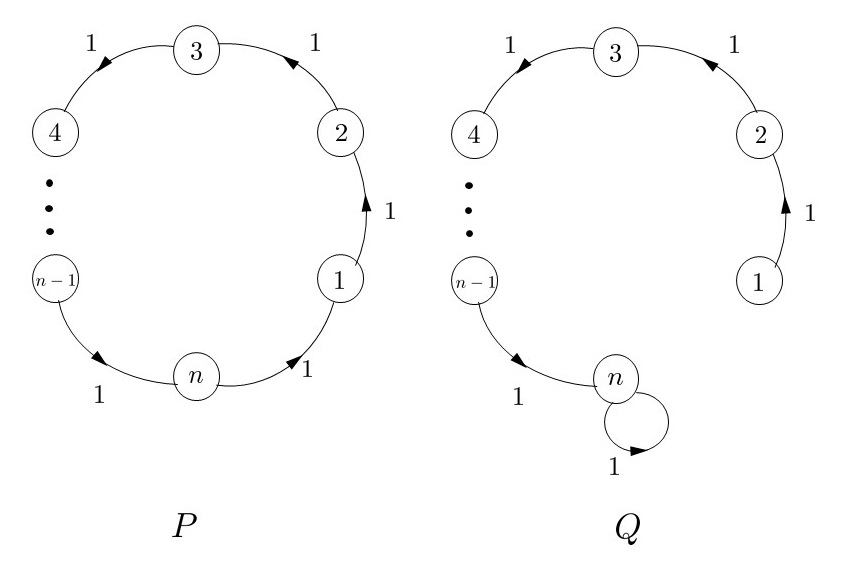
\includegraphics[scale=0.40]{diagrams/example2.jpg}
%	\caption{Example 2.}
%	\label{fig:example2}
%\end{figure}
%\end{example}
%
%\begin{example}
%\label{example:stationary_testing}
%Non symmetric MC: small difference between $P$ and $Q$ ($\dist{\word{P}{\ell}}{\word{Q}{\ell}}$ is small), but stationary distributions $\vect{p}_0$ and $\vect{q}_0$
%are vastly different. $Q$ - a ring with an edge $e=(v_1v_2)$ is removed, $v_1$ has a self-loop instead; $P$ - a similar ring with a loop, but $e$ is not removed but has a lighter
%weight of $\frac{1}{\sqrt{n}}$, while self-loop at $v_1$ has a weight of $1-\frac{1}{\sqrt{n}}$. Stationary distributions: $\vect{q}_0=\trans{(1,0,\cdots,0)}$ and
%$\vect{p}_0=\trans{(\frac{\sqrt{n}}{n+\sqrt{n}-1},\frac{1}{n+\sqrt{n}-1},\dots,\frac{1}{n+\sqrt{n}-1})}$, while $\specr{\srprod{P}{Q}}=\sqrt{1-\frac{1}{\sqrt{n}}}$.   
%%\begin{figure}[H]
%	%\centering
%		%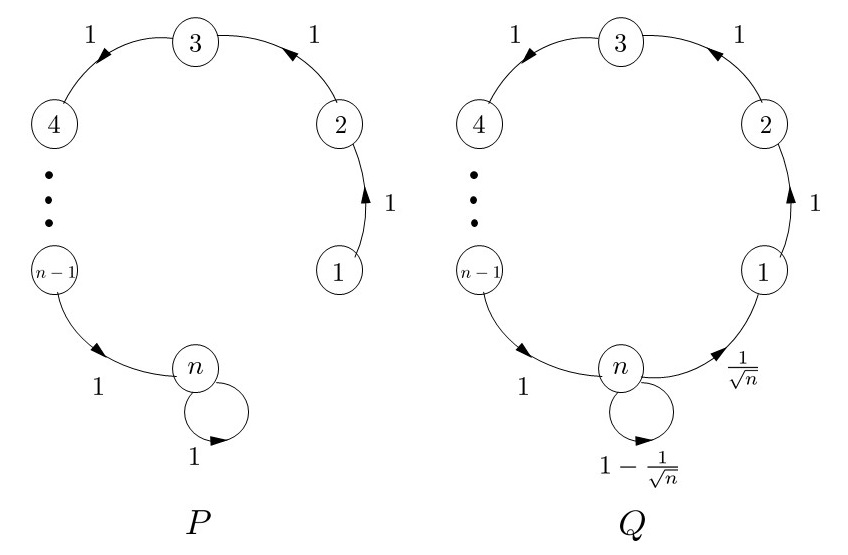
\includegraphics[scale=0.40]{diagrams/example3.jpg}
%	%\caption{Example 3.}
%	%\label{fig:example3}
%%\end{figure}
%
%\end{example}
%\begin{example}
%\label{example:same_stationary_large_dist}
%Non symmetric MC: same stationary (Uniform) distribution, $\dist{P}{Q}=1$, at average it takes $\Omega(n)$ steps to distinguish whether $P=Q$, or not.
%Two oriented cycles, 
%\[
%P\eqdef s_1\to s_2\to\cdots\to s_n\to s_1\quad\quad Q\eqdef s_1\to s_3\to s_4\cdots\to s_n\to s_2\to s_1.
%\]
%%\begin{figure}[H]
%	%\centering
%		%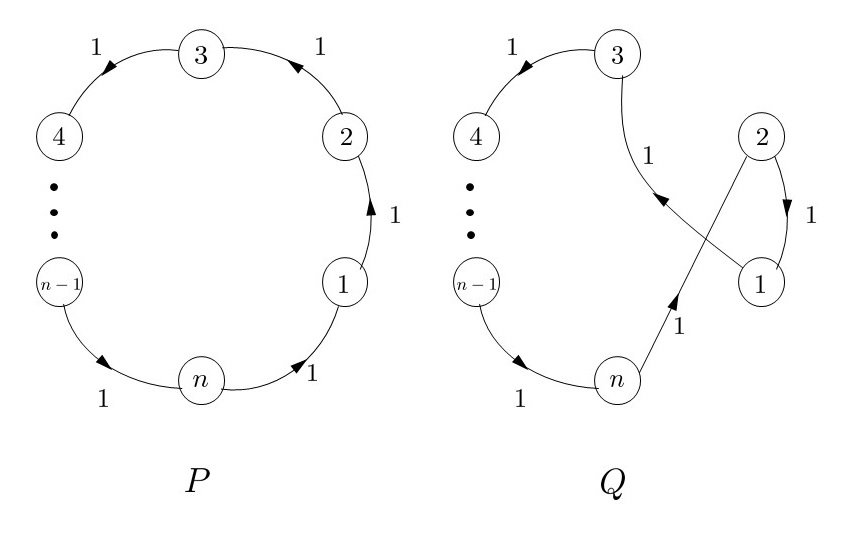
\includegraphics[scale=0.40]{diagrams/example4.jpg}
%	%\caption{Example 4.}
%	%\label{fig:example4}
%%\end{figure}
%\end{example}
%\begin{example}
%\label{example:symmetric}
%Symmetric Markov chains: $Q$ -- complete graph $Q_{ij}=1/n$; $P$ -- clique and disjoint vertex $P_{ij}=\frac{1}{n-1}, i,j\in[n-1]$, $P_{in}=P_{ni}=0, i\in[n-1],$ and 
%$P_{nn}=1$. Then $\eigi[1]=\sqrt{\frac{n-1}{n}}= 1 - \frac{1}{2n}+O(n^2)$, $\eigi[2]=\sqrt{\frac{1}{n}}$, $\eigi[3]=\cdots=\eigi[n]=0$. If Markov Chain starts from state $1$, 
%after one transition we would know almost certainly whether $w\sim P$, or $w\sim Q$. On the other hand, if $w$ starts from any other state, then it would take us about $n$ 
%observations to tell whether $w\sim P$, or $w\sim Q$. If we start from a random state, again we would need about $n$ steps to distinguish $P$ vs. $Q$.
%%\begin{figure}[H]
%	%\centering
%		%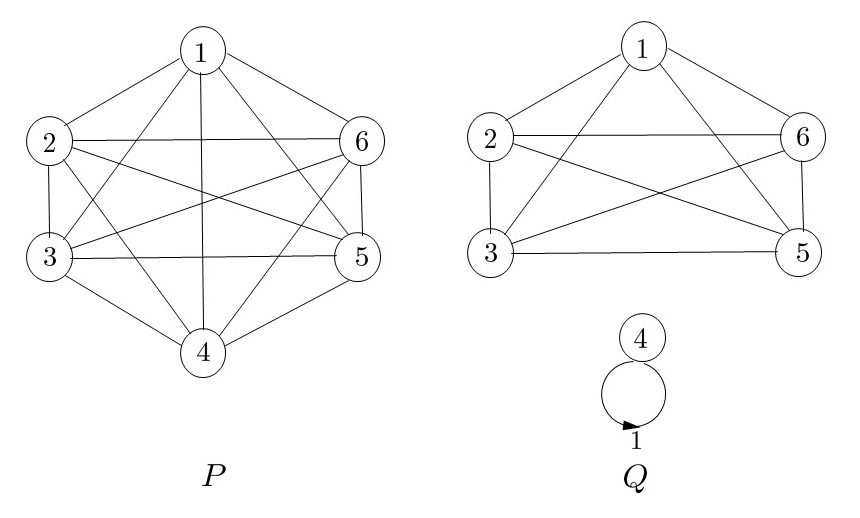
\includegraphics[scale=0.40]{diagrams/example5.jpg}
%	%\caption{Example 5.}
%	%\label{fig:example5}
%%\end{figure}
%\end{example}






% Acknowledgments---Will not appear in anonymized version
\acks{This work was supported by grants from the MITEI-Shell program, Amazon Research Award and Simons Investigator Award.}


\bibliography{sublinear_space_nn}

\newpage
\appendix
\section{Deferred Proofs from Section~\ref{sec:sketch}}\label{sec:sketch_proofs}

\begin{proof}[Proof of Lemma~\ref{lmm:tree_size}]
Charging the degree-$1$ nodes along every maximal $1$-path to its bottom (non-degree-$1$) node,
the total number of nodes after top-out compression is bounded by
\[ \sum_{v:\mathrm{deg}(v)\neq1}\Lambda(v) . \]
\cite{indyk2017near} show this is at most $O(n\log(1/\epsilon))$.
The difference is that their compression replaces summands larger than $\Lambda(v)$ by zero, while our (top-out) compression trims them to $\Lambda(v)$.
%The upper bound holds in both cases.
\end{proof}


\begin{proof}[Proof of Lemma~\ref{lmm:subtree_root}]
By top-out compression, $v$ is the top of a downward $1$-path of length $\Lambda(v')$ whose bottom node is $v'$. Since no clusters are joined along a $1$-path, we have $C(v')=C(v)$, hence $x,x'\in C(v')$ and hence $\norm{x-x'} \leq \Delta(v')$. 
Noting that $\ell(v)=\ell(v')+\Lambda(v')=\ell(v')+\log(\Delta(v')/(2^{\ell(v')}\epsilon))=\log(\Delta(v')/\epsilon)$ and rearranging, we find $\Delta(v')=2^{\ell(v)}\epsilon$, which yields the claim.
\end{proof}


\begin{proof}[Proof of Lemma~\ref{lmm:subtree_leaf}]
If $u$ is a leaf in $T$ then $C(u)$ is a singleton cluster, hence $x=x'$.
Otherwise $u$ is the top node of a long edge, and the claim follows by Lemma~\ref{lmm:subtree_root} on the bottom node of that long edge.
\end{proof}


\begin{proof}[Proof of Lemma~\ref{lmm:surrogates}]
The first part of the lemma (where $v$ is any node, not necessarily a subtree leaf) is proved by induction on the ingresses.
In the base case we use that $\norm{x_{c(v)}-s^*(v)}\leq2^{\ell(v)}$ by the choice of grid net.
The induction step is identical to~\cite{indyk2017near}.
The ``furthermore'' part of the lemma then follows as a corollary due to the refined definition of $\gamma(v)$ for a subtree leaf $v$, in the induction step leading to it.
\end{proof}



\begin{proof}[Proof of Lemma~\ref{lmm:sketch_size}]
The sketch of~\cite{indyk2017near} stores the compressed tree $T'$, with each node annotated by its center $c(v)$, ingress $\mathrm{in}(v)$, precision $\gamma(v)$ and quantized displacement $\eta(v)$.
Every long edge is annotated by its length.
They show this takes
\[ O\left( n\left((d+\log n)\log(1/\epsilon) + \log\log\Phi\right)\right) \]
bits;
note that by Lemma~\ref{lmm:tree_size}, top-out compression did not effect this bound.

We additionally store the hashed surrogates of subtree roots.
There are $O(n)$ subtrees,\footnote{By construction, the tree of subtrees in $T$ has no degree-$1$ nodes. Since $T$ has $n$ leaves, there are at most $2n-1$ subtrees.} and each hash takes $\log m$ bits to store, which adds $O(n(d+\log\log\Phi+\log(q/\delta)))$ bits to the above.
Finally, we store the hash functions $H_\ell$ for every $\ell$.
The domain of each $H_\ell$ is $N_{2^\ell}$, which is a subset of $\{-\Phi \ldots \Phi\}^d$, and hence $H_\ell$ can be specified by $O(\log(\Phi^d))$ random bits (\cite{carter1979universal}).
Since we do not require independence between hash functions of different levels, we can use the same random bits for all hash functions, adding a total of $O(d\log\Phi)$ bits to the sketch.
\end{proof}


\section{Approximate Nearest Neighbor Sketching Lower Bound}\label{sec:nnlower}

\begin{theorem}\label{thm:ann_lb}
Suppose that $d\geq\Omega(\epsilon^{-2}\log n)$, $\Phi\geq1/\epsilon$, and $1/n^{0.5-\beta}\leq\epsilon\leq\epsilon_0$ for a constant $\beta>0$ and a sufficiently small constant $\epsilon_0$.
Suppose also that $\delta<1/n^2$.
Then, for the all-nearest-neighbors problem, Alice must use a sketch of at least $\Omega(\beta\epsilon^{-2}n\log n)$ bits.
\end{theorem}
\begin{proof}
We start with dimension $d=n+1+\log n$; it can then be reduced by standard dimension reduction.
Fix $k=1/\epsilon^2$ and assume w.l.o.g.~that $k$ is a square integer (by taking $\epsilon$ to be appropriately small). Note that since $\epsilon>1/\sqrt{n}$ we have $k\leq n$, and that since $\Phi\geq1/\epsilon$ we have $\sqrt{k}\leq\Phi$. 

The data set will consist of $2n$ points, $x_1,\ldots,x_n$ and $z_1,\ldots,z_n$.
Let $i\in[n]$. We choose the first $n$ coordinates of $x_i$ to be an arbitrary $k$-sparse vector, in which each nonzero coordinate equals $1/\sqrt{k}$. Note that the norm of this part is $1$. The $(n+1)$th coordinate of $x_i$ is set to $0$. The remaining $\log n$ coordinates encode the binary encoding of $i$, with each coordinate multiplied by $10$.

Next we define $z_i$. The first $n$ coordinates are $0$. The $(n+1)$th coordinate equals $\sqrt{1-\epsilon}$. The remaining $\log n$ coordinates encode $i$ similarly to $x_i$.

The number of different choices for $\{x_1,\ldots,x_n\}$ is ${n\choose k}^n$.
Therefore if we show that one can fully recover $x_1,\ldots,x_n$ from a given all-nearest-neighbor sketch of the dataset, we would get the desired lower bound
\[
  \log\left({n\choose k}^n\right) \geq
   nk\log(n/k) = \epsilon^{-2}n\log(\epsilon^2n) =\epsilon^{-2}n\log(n^{2\beta}) = 2\beta\epsilon^{-2}n\log n .
\]

Suppose we have such a sketch.
For given $i,j\in[n]$ we now show how to recover the $j$th coordinate of $x_i$, denoted $x_i(j)$, with a single approximate nearest neighbor query.
Let $y_{ij}$ be the following vector in $\R^d$: The first $n+1$ coordinates are all zeros, except for the $j$th coordinate which is set to $1$. The last $\log n$ coordinates encode $i$ similary to $x_i$ and $z_i$.

Consider the distances from $y_{ij}$ to all data points. We start with $x_i$. It is identical to $y_i$ in the last $\log n+1$ coordinates, so we will restrict both to the first $n$ coordinates and denote the restricted vectors by $x_i^{:n}$ and $y_{ij}^{:n}$. $x_i^{:n}$ is a $k$-sparse vector with nonzero entries equal to $1/\sqrt{k}$, hence $\norm{x_i^{:n}}=1$. $y_{ij}^{:n}$ is just the standard basis vector $e_j$ in $\R^n$. Hence,
\[
  \norm{x_i-y_{ij}}^2 =
  \norm{x_i^{:n}-y_{ij}^{:n}}^2 =
  \norm{x_i^{:n}}^2 + \norm{y_{ij}^{:n}}^2 - 2(x_i^{:n})^\top y_{ij}^{:n} =
  2-2x_i(j).
\]
This equals $2$ if $x_i(j)=0$ and $2-2/\sqrt k=2-2\epsilon$ if $x_i(j)=1/\sqrt k$.

Next consider $z_i$. It is identical to $y_{ij}$ in all except the $j$th coordinate, which is $0$ in $z_i$ and $1$ in $y_{ij}$, and the $(n+1)$th coordinate, which is $0$ for $y_{ij}$ and $\sqrt{1-\epsilon}$ for $z_i$. Therefore, $\norm{z_i-y_{ij}}^2=2-\epsilon$.

Finally, for every $i'\neq i$, both $x_{i'}$ and $z_{i'}$ are at distance at least $10$ from $y_{ij}$ due to the encoding of $i$ (as binary multiplied by $10$) in the last $\log n$ coordinates.

In summation we have established the following:
\begin{itemize}
  \item If $x_i(j)\neq0$, then the closest point to $y_{ij}$ in the dataset is $x_i$ at distance $\sqrt{2-2\epsilon}$, and the next closest point is $z_i$ at distance $\sqrt{2-\epsilon}$.
  \item If $x_i(j)=0$, then the closest point to $y_{ij}$ in the dataset is $z_i$ at distance $\sqrt{2-\epsilon}$, and the next closest point is $x_i$ at distance $2$.
\end{itemize}
Therefore, if the sketch supports $(1+\frac{1}{8}\epsilon)$-approximate nearest neighbors, we can recover the true nearest neighbor of $y_{ij}$ and thus recover $x_i(j)$. By hypothesis, the query succeeds with probability $\delta<1/n^2$.
By a union bound over all $i,j\in[n]$ we can recover all of $x_1,\ldots,x_n$ simultaneously, and the theorem follows.
\end{proof}
\newcommand{\Rlin}{R^{\mathrm{lin}}}
\section{Lower bound}
\label{s:lower}
In this section we derive a lower bound for bandits with composite anonymous feedback. We do that through a reduction from the setting of linear bandits (in the probability simplex) to our setting. This reduction allows us to upper bound the regret of a linear bandit algorithm in terms of (a suitably scaled version of) the regret of an algorithm in our setting. Since the reduction applies to any instance of a linear bandit problem, we can use a known lower bound for the linear bandit setting to derive a corresponding lower bound for our composite setting.

Let $\Delta_K$ be the probability simplex in $\R^K$. At each round $t$, an algorithm $A$ for linear bandit optimization chooses an action $\bp_t\in\Delta_K$ and suffers loss $\bloss_t^{\top}\bp_t$, where $\bloss_t \in [0,1]^K$ is some unknown loss vector. The feedback observed by the algorithm at the end of round $t$ is the scalar $\bloss_t^{\top}\bp_t$. The regret suffered by algorithm $A$ playing actions $\bp_1,\dots,\bp_T$ is
\begin{equation}
\label{eq:lin-regret}
	\Rlin_T = \sum_{t=1}^T \bloss_t^{\top}\bp_t - \min_{\bp\in\Delta_K} \sum_{t=1}^T \bloss_t^{\top}\bp = \sum_{t=1}^T \bloss_t^{\top}\bp_t - \min_{i=1,\dots,K} \sum_{t=1}^T \loss_t(i)
\end{equation}
where we used the fact that a linear function on the simplex is minimized at one of the corners.
Let $\Rlin_T(A,\Delta_K)$ denote the worst case regret (over the oblivious choice of $\bloss_1,\dots,\bloss_T$) of algorithm $A$. Similarly, let $R_T(A_d,K,d)$ be the worst case regret (over the oblivious choice of loss components $\loss_t^{(s)}(i)$ for all $t$, $s$, and $i$) of algorithm $A_d$ for nonstochastic $K$-armed bandits with $d$-delayed composite anonymous feedback. Our reduction shows the following.
%
\begin{lemma}\label{lem:lower}
For any algorithm $A_d$ for $K$-armed bandits with $d$-delayed composite anonymous feedback, there exists an algorithm $A$ for linear bandits in $\Delta_K$ such that
$
	R_T(A_d,K,d) \ge d\,\Rlin_{T/d}(A,\Delta_K)
$.
\end{lemma}
%
%
Our reduction, described in detail in the proof of the above lemma (see the appendix), essentially builds the probability vectors $\bp_t$ played by $A$ based on the empirical distribution of actions played by $A_d$ during blocks of size $d$. Now, an additional lemma is needed (whose proof is given in the appendix).
\begin{lemma}
\label{l:shamir}
The regret of any algorithm $A$ for linear bandits in the simplex satisfies $\Rlin_T(A,\Delta_K) = \widetilde{\Omega}\big(\sqrt{KT}\big)$.
\end{lemma}
%
Using the above two lemmas we can prove the following theorem.
\begin{theorem}
For any algorithm $A_d$ for $K$-armed bandits with $d$-delayed composite anonymous feedback,
$
R_T(A_d,K,d)=\widetilde{\Omega}\big(\sqrt{dKT}\big)
$.
\end{theorem}
%
\begin{proof}
Fix an algorithm $A_d$. Using the reduction of~Lemma~\ref{lem:lower} gives an algorithm $A$ such that
$
	R_T(A_d,K,d) \ge d\,\Rlin_{T/d}(A,\Delta_K) = \widetilde{\Omega}\big(\sqrt{dKT}\big)
$,
where we used Lemma~\ref{l:shamir} with horizon $T/d$ to prove the $\widetilde{\Omega}$-equality.
\end{proof}
%
Although the loss sequence used to prove the lower bound for linear bandits in the simplex is stochastic i.i.d., the loss sequence achieving the lower bound in our delayed setting is not independent due to the deterministic loss transformation in the proof of Lemma~\ref{lem:lower} (which is defined independent of the algorithm, thus preserving the oblivious nature of the adversary).


\section{Practical Variant}\label{sec:middleout}
\cite{indyk2017practical} presented a simplified version of the sketch of~\cite{indyk2017near}, which is lossier by a factor $O(\log\log n)$ in the size bound (more precisely it uses $O(\epsilon^{-2}\log(n)(\log\log(n) + \log(1/\epsilon))+\log\log\Phi)$ bits per point; compare this to Table~\ref{tbl:sketches_related_work}), but on the other hand is practical to implement and was shown to work well empirically.
Both variants do not provably support out-of-sample queries.

In the main part of this work, we showed how to adapt the framework of~\cite{indyk2017near} to support out-of-sample queries with nearly optimal size bounds.
The goal of this section is to show that our techniques can also be applied in a simplified way to~\cite{indyk2017practical} in order to obtain a~\emph{practical} algorithm.
Specifically, focusing on the all-nearest-neighbors problem, we will show that a slight modification to~\cite{indyk2017practical} yields provable support in out-of-sample approximate nearest neighbor queries, with a size bound that is the same as in Theorem~\ref{thm:ann_ub} plus an additive $O(\epsilon^{-2}\log(n)\log\log(n))$ term.

\paragraph{Technique: Middle-out compression}
In~\cite{indyk2017practical}, every $1$-path is pruned (i.e.~replaced by a long edge) except for its top $\Lambda$ nodes, where $\Lambda$ is an integer parameter.
Combining this ``bottom-out'' compression with the ``top-out'' compression which was introduced in Section~\ref{sec:sketch}, we obtain~\emph{middle-out compression}: every long $1$-path longer than $2\Lambda$ is replaced by a long edge, except for its top and bottom $\Lambda$ nodes.
As we will show in the remainder of this section, applying this pruning rule to the quadtree of~\cite{indyk2017practical} (instead of their ``bottom-out'' rule) is sufficient to obtain a sketch that provably supports out-of-sample approximate nearest neighbor queries. Thus, the sketching algorithm is nearly unchanged.

We remark that in Section~\ref{sec:sketch} we introduced two additional modifications: \emph{grid-net quantization} and~\emph{surrogate hashing}. These were required in order to prove Theorems~\ref{thm:ann_ub} and~\ref{thm:distances_ub}, but in the framework of~\cite{indyk2017practical} they turn out to be unnecessary: grid-net quantization is already organically built into the quadtree approach of~\cite{indyk2017practical}, and surrogate hashing only served to avoid a $O(\log\log n)$ factor in the sketch size (see footnote 4), but in~\cite{indyk2017practical} this factor is tolerated anyway.

\subsection{Sketching Algorithm Recap}
For completeness, let us briefly describe the sketching algorithm of~\cite{indyk2017practical} (the reader is referred to that paper for more formal details), with our modification.
To this end, set
\[ \Lambda = \lceil\log\left(\frac{16d^{1.5}\log\Phi}{\epsilon\delta}\right)\rceil . \]
Suppose w.l.o.g.~that $\Phi$ is a power of $2$. The sketching algorithm proceeds in three steps:
\begin{enumerate}
  \item\emph{Random shifted grids:} Impose a randomly shifted enclosing hypercube on the data points $X$. More precisely, choose a uniformly random shift $\sigma\in\{-\Phi,\ldots,\Phi\}^d$, and set the enclosing hypercube to be $H=[-2\Phi+\sigma_1,2\Phi+\sigma_1]\times[-2\Phi+\sigma_2,2\Phi+\sigma_2]\times\ldots\times[-2\Phi+\sigma_d,2\Phi+\sigma_d]$. Since $X\subset\{-\Phi,\ldots,\Phi\}^d$, it is indeed enclosed by $H$. We then half $H$ along every dimension to create a finer grid with $2^d$ cells, and proceed so (recursively halving every cell along every dimension) to create a hierarchy of nested grids, with $\log(4\Phi)+\Lambda$ hierarchy levels. The top level is numbered $\Phi+2$, which is the log the side length of $H$, and the next levels are decrementing, so  that the grid cells in level $\ell$ have side length $2^\ell$.
  \item\emph{Quadtree construction:} Construct the quadtree which is naturally associated with the nested grids: the root corresponds to $H$, its children correspond to the non-empty cells of the next grid in the hierarchy (a cell is non-empty if it contains a point in $X$), and so on.
Each tree edge is annotated by a bitstring of length $d$, that marks whether the child cell coincides with the bottom half (bit $0$) or the top half (bit $1$) of the parent cell in each dimension.
  \item\emph{Middle-out compression:} For every path of degree-$1$ tree nodes whose length is more than $2\Lambda$, we keep its top $\Lambda$ and bottom $\Lambda$, and replace its remaining middle portion by a long edge. This removes the edge annotations of the middle section (this achieving compression). We label each long edge with the length of the path it replaces.
\end{enumerate}

In the remainder of this section we prove the following.
\begin{theorem}\label{thm:ann_practical}
The above algorithm, with the above setting of $\Lambda$, runs in time $\tilde O(nd(\log\Phi+\Lambda))$ and produces a sketch for the all-nearest-neighbors problem, whose size in bits is
\[
  O\left( n\left(\frac{\log n\cdot(\log\log n + \log(1/\epsilon))}{\epsilon^2} + \log\log\Phi + \log\left(\frac{q}{\delta}\right)\right) + d\log\Phi  + \log\left(\frac{q}{\delta}\right)\log\left(\frac{\log(q/\delta)}{\epsilon}\right) \right).
\]
\end{theorem}

The sketch size is the same as in~\cite{indyk2017practical}, except that we keep at most $2\Lambda$ instead of $\Lambda$ nodes per $1$-path, which increases the sketch size by only a factor of $2$.

\subsection{Basic lemmas}
We start with some useful properties of the above sketch, which are analogous to lemmas from in Section~\ref{sec:sketch}. In the notation below, for a node $v$ in the quadtree, $C(v)$ denotes the subset of points in $X$ that are contained in the grid cell associated with $v$. As in Section~\ref{sec:sketch}, the quadtree is partitioned into a set $\mathcal F(T)$ of~\emph{subtrees} by removing the long edges.

\begin{lemma}[analog of Lemma~\ref{lmm:separation}]\label{lmm:separation_quadtree}
For every point $x\in X$, with probability $1-\delta$, the following holds.
If $z\in\R^d$ is any point outside the grid cell that contains $x$ in level $\ell$ of the quadtree, then $\norm{x-x'}\geq 8\epsilon^{-1}\cdot2^{\ell-\Lambda}\sqrt{d}$.
\end{lemma}
\begin{proof}
The setting of $\Lambda$ is such that with probability $1-\delta$, in every level $\ell$ of the quadtree, the grid cell that contains $x$ also contains the ball at radius $8\epsilon^{-1}\cdot2^{\ell-\Lambda}\sqrt{d}$ around $x$. (This property is known as ``padding''.) The lemma is just a restatement of this property.
See Lemma 1 and Equation (1) in~\cite{indyk2017practical} for details.
\end{proof}

\begin{lemma}[analog of Lemmas~\ref{lmm:subtree_root}, \ref{lmm:subtree_leaf}, \ref{lmm:surrogates}]\label{lmm:samecell}
Let $v$ be a node in the quadtree, and $x,x'\in\R^d$ points contained in the grid cell associated with $v$. Then $\norm{x-x'}\leq2^{\ell(v)}\sqrt{d}$.
\end{lemma}
\begin{proof}
The grid cell associated with $v$ is a hypercube with side $2^{\ell(v)}$ and diameter $2^{\ell(v)}\sqrt{d}$.
\end{proof}

Before proceeding let us make the following point about the quadtree.
\begin{claim}\label{clm:quadtree_levels}
For every leaf $v$ of the quadtree, $C(v)$ contains a single point of $X$, and $v$ is the bottom of a $1$-path of length at least $\Lambda$.
\end{claim}
\begin{proof}
Refining the quadtree grid hierarchy for $\log(4\Phi)$ levels ensures that each grid cell contains at most one point from $X$, and refining for $\Lambda$ additional levels ensures that each leaf is the bottom of a $1$-path of length at least $\Lambda$.
\end{proof}

\begin{claim}\label{clm:leaves}
Every subtree leaf in the quadtree is the bottom of a $1$-path of length at least $\Lambda$.
\end{claim}
\begin{proof}
If $v$ is a leaf of the quadtree, this follows from Claim~\ref{clm:quadtree_levels}. Otherwise this follows from middle-out compression.
\end{proof}

Next we define centers and surrogates.
Centers $c(v)$ are chosen similarly to Section~\ref{sec:sketch}.
The surrogate $s^*(v)$ of every tree node $v$ is simply defined to be the ``bottom-left'' (i.e.~minimal in all dimensions) corner of the grid cell associated with $v$.

\subsection{Approximate Nearest Neighbor Search}
Finally, we can describe the query algorithm and complete its analysis.
Let $y$ be a query point for which we need to report an approximate nearest neighbor from the sketch. The query algorithm is the same as in Section~\ref{sec:ann}: starting with the subtree that contains the quadtree root, it recovers the surrogates in the current subtree and chooses the subtree $v$ whose surrogate is the closest to $y$. If $v$ is a quadtree leaf, its center is returned as the approximate nearest neighbor. Otherwise, the algorithm proceeds by recursion on the subtree under $v$.

\paragraph{Surrogate recovery}
The difference is in the way we recover the surrogates of a given subtree. In Section~\ref{sec:ann} this was done using the surrogate hashes. Here we will use a simpler, deterministic surrogate recovery subroutine.
Let $s^*(H)\in\R^d$ the surrogate of the quadtree root. (We store this point explicitly in the sketch, and it will be convenient to think of it w.l.o.g.~as the the origin in $\R^d$.) As observed in~\cite{indyk2017practical}, for every tree node $v$, if we concatenate the bits annotating the edges on the path from the root to $v$, we get the binary expansion of the point $s^*(H)+s^*(v)$. Therefore, we can recover $s^*(v)$ from the sketch, as long as the path from the root to $v$ does not traverse a long edge.

If the path to $v$ contains long edges (and thus missing bits in the binary expansion of $s^*(v)$), the algorithm completes these bits from the binary expansion of $y$.
Let $r_0,r_1,\ldots$ be the subtree roots traversed by the algorithm, and let $T_0,T_1,\ldots$ be the corresponding subtrees. Let $t$ be the smallest such that the algorithm does not recover the surrogates in $T_t$ correctly (because the bits missing on the long edge connecting $T_{t-1}$ to $T_t$ are not truly equal to those of $y$). As in Section~\ref{sec:ann}, the query algorithm does not know $t$ (it simply always assumes that the bits of $y$ are the correct missing ones), but we will use it for analysis.
Note that by definition of $t$, all surrogates in the subtrees rooted at $r_0,\ldots,r_{t-1}$ are recovered correctly. Thus, the event from Lemma~\ref{lmm:hashes} holds deterministically.

\paragraph{Proof of Theorem~\ref{thm:ann_practical}}
Let $x^*\in X$ be a fixed true nearest neighbor of $y$ in $X$ (chosen arbitrarily if there is more than one). We shall assume that the event in Lemma~\ref{lmm:separation_quadtree} occurs for $x^*$.

\begin{lemma}[analog of Lemma~\ref{lmm:annrounds}]\label{lmm:annrounds_quadtree}
Let $T'\in\mathcal F(T)$ be a subtree rooted in $r$, such that $x^*\in C(r)$.
Let $v$ a leaf of $T'$ that minimizes $\norm{y-s^*(v)}$.
Then either $x^*\in C(v)$,
or every $z\in C(v)$ is a $(1+O(\epsilon))$-approximate nearest neighbor of $y$.
\end{lemma}
\begin{proof}
If $x^*\in C(v)$ then we are done. Assume now that $x^*\in C(u)$ for a leaf $u\neq v$ of $T'$.
Let $\ell:=\max\{\ell(v),\ell(u)\}$. We start by showing that $\norm{y-x^*}>\epsilon^{-1}2^\ell\sqrt{d}$.
Assume by contradiction this is not the case.
Since $x^*\in C(u)$ we have $\norm{x^*-x_{c(u)}}\leq2^{\ell}\sqrt{d}$ by Lemma~\ref{lmm:samecell}, and similarly $\norm{x_{c(u)}-s^*(u)}\leq2^{\ell}\sqrt{d}$. Together, $\norm{y-s^*(u)}\leq(\epsilon^{-1}+2)2^\ell\sqrt{d}$.
On the other hand, by the triangle inequality,
$\norm{y-s^*(v)} \geq \norm{x^*-x_{c(v)}} - \norm{y-x^*} - \norm{x_{c(v)}-s^*(v)}$.
By Claim~\ref{clm:leaves}, both $v$ and $u$ are the bottom of $1$-paths of length at least $\Lambda$, This means that $x^*$ and $x_{c(v)}$ are separated already at level $\ell+\Lambda$, and by Lemma~\ref{lmm:separation_quadtree} this implies $\norm{x^*-x_{c(v)}}\geq8\epsilon^{-1}\cdot2^{\ell}\sqrt{d}$. By the contradiction hypothesis we have $\norm{y-x^*}\leq\epsilon^{-1}2^\ell\sqrt{d}$, and by Lemma~\ref{lmm:samecell}, $\norm{x_{c(v)}-s^*(v)}\leq2^\ell\sqrt{d}$. 
Putting these together yields $\norm{y-s^*(v)}\geq8\epsilon^{-1}\cdot2^{\ell}\sqrt{d}-\epsilon^{-1}2^\ell\sqrt{d}-2^\ell\sqrt{d} > (\epsilon^{-1}+2)2^\ell\sqrt{d}\geq \norm{x_{c(u)}-s^*(u)}$. This contradicts the choice of $v$.

The lemma now follows because for every $z\in C(v)$,
\begin{align}
\norm{y-z} &\leq \norm{y-s^*(v)} + \norm{s^*(v)-x_{c(v)}} + \norm{x_{c(v)}-z} \label{ineq1b} \\
&\leq \norm{y-s^*(u)} + \norm{s^*(v)-x_{c(v)}} + \norm{x_{c(v)}-z} \label{ineq2b} \\
&\leq \norm{y-x^*} + \norm{x^*-x_{c(u)}} + \norm{x_{c(u)}-s^*(u)} +\norm{s^*(v)-x_{c(v)}} + \norm{x_{c(v)}-z} \label{ineq3b} \\
&\leq \norm{y-x^*} + 4\cdot2^\ell\sqrt{d} \label{ineq4b} \\
&\leq (1+4\epsilon)\norm{y-x^*}, \label{ineq5b}
\end{align}
where~(\ref{ineq1b}) and (\ref{ineq3b}) are by the triangle inequality, (\ref{ineq2b}) is since $\norm{y-s^*(v)}\leq\norm{y-s^*(u)}$ by choice of $v$, (\ref{ineq4b}) is by applying Lemma~\ref{lmm:samecell} to each of the last four summands, and~(\ref{ineq5b}) is since we have shown that $\norm{y-x^*}>\epsilon^{-1}2^\ell\sqrt{d}$.
Therefore $z$ is a $(1+4\epsilon)$-approximate nearest neighbor of $y$.
\end{proof}

Now we prove that the query algorithm returns an approximate nearest neighbor for $y$.
We may assume w.l.o.g.~that $\epsilon$ is smaller than a sufficiently small constant.
We consider two cases. In the first case, $x^*\notin C(r_t)$.
Let $i\in\{1,\ldots,t\}$ be the smallest such that $x^*\notin C(r_i)$.
By applying Lemma~\ref{lmm:annrounds_quadtree} on $r_{i-1}$, we have that every point in $C(r_i)$ is a $(1+O(\epsilon))$-approximate nearest neighbor of $y$. After reaching $r_i$, the algorithm would return the center of some leaf reachable from $r_i$, and it would be a correct output.

In the second case, $x^*\in C(r_t)$ contains a true nearest neighbor of $y$. We will show that every point in $C(r_t)$ is a $(1+O(\epsilon))$-approximate nearest neighbor of $y$, so once again, once the algorithm arrives at $r_t$ it can return anything.
By definition of $t$, we know that $y$ does not reside in the grid cell associated with $r_t$. Since $y$ does reside in that cell, we have $\norm{y-x^*}\geq8\epsilon^{-1}2^{\ell(r_t)-\Lambda}\sqrt{d}$ by Lemma~\ref{lmm:separation_quadtree}. On the other hand, by Claim~\ref{clm:leaves}, $r_t$ is the bottom of a $1$-path of length at least $\Lambda$, and therefore any two points in $C(r_t)$ are contained in the same grid cell at level $\ell(r_t)-\Lambda$, whose diameter is $2^{\ell(r_t)-\Lambda}\sqrt{d}$. In particular, for every $x\in C(r_t)$ we have $\norm{x-x^*}\leq2^{\ell(r_t)-\Lambda}\sqrt{d}\leq\frac{1}{8}\epsilon\norm{y-x^*}$. Altogether we get $\norm{y-x} \leq \norm{y-x^*} + \norm{x^*-x} \leq (1+\frac{1}{8}\epsilon)\norm{y-x^*}$, so every $x\in C(r_t)$ is a $(1+\epsilon)$-approximate nearest neighbor of $y$ in $X$.

The proof assumes the event in Lemma~\ref{lmm:separation_quadtree} holds for $x^*$, which happens with probability $1-\delta$. To handle $q$ queries, we can scale $\delta$ down to $\delta/q$ and take a union bound over the $q$ nearest neighbors of the $q$ query points \qed


\end{document}
